% =============================================================================
% IEEEtran source for the DS108 Electrimight report
% =============================================================================
\documentclass[conference]{IEEEtran}
\IEEEoverridecommandlockouts

% ---------- Vietnamese Support ----------
\usepackage[utf8]{inputenc}
\usepackage[T5]{fontenc}
\usepackage[vietnamese]{babel}
\addto\captionsvietnamese{%
  \def\tablename{TABLE}%
  \def\figurename{Fig.}%
}

% ---------- Packages ----------
\usepackage{cite}
\usepackage{amsmath,amssymb,amsfonts}
\usepackage{algorithm}
\usepackage{algorithmic}
\usepackage{graphicx}
\usepackage{textcomp}
\usepackage{xcolor}
\usepackage{booktabs}
\usepackage{multirow}
\usepackage{longtable}
\usepackage{pgfplots}
\pgfplotsset{compat=1.17}
\usepackage{subcaption}

% ---------- Hyphenation ----------
\hyphenation{op-tical net-works semi-conduc-tor}

% ---------- Document ----------
\begin{document}

% ---------- Title ----------
\title{Xây dựng Dataset Giàu Đặc trưng cho Phân tích Tiêu thụ Điện Công nghiệp Ngành Thép}

% ---------- Authors ----------
\author{
    \IEEEauthorblockN{Hoàng Nguyễn Minh Khang\textsuperscript{1},
    Nguyễn Sỹ Huỳnh\textsuperscript{1}}
    \IEEEauthorblockA{\textsuperscript{1}\textit{Trường Đại học Công nghệ Thông tin},
    ĐHQG Thành phố Hồ Chí Minh, Việt Nam}
}

\maketitle

% ---------- Abstract ----------
\begin{abstract}
Dự báo tiêu thụ điện năng công nghiệp và phân loại rủi ro đòi hỏi dataset có chất lượng cao, schema rõ ràng và đặc trưng đủ giàu để hỗ trợ kiểm toán. Bài báo này trình bày một pipeline tiền xử lý cho tập dữ liệu Steel Industry Energy Consumption, một chuỗi thời gian công nghiệp được ghi nhận tại nhà máy thép Hàn Quốc. Pipeline kết hợp feature engineering miền thời gian, đặc trưng miền tần số bằng Discrete Wavelet Transform (DWT) với wavelet Daubechies-4, weather enrichment từ Open-Meteo và các đặc trưng physics-informed như apparent power và phase angle. Ba nhóm proxy anomaly labels cho idle load, energy leakage và local overload được xây dựng bằng ngưỡng vật lý có giải thích, đồng thời một module GAN dạng bảng được khảo sát như hướng tăng cường dữ liệu cho lớp thiểu số. Gold dataset sau xử lý gồm 35.040 bản ghi và 69 cột, mở rộng từ 11 cột gốc bằng các lớp đặc trưng thời gian, thời tiết, wavelet, vật lý, nhãn và confidence score. Kết quả ablation cho thấy đóng góp chính của nghiên cứu nằm ở việc xây dựng một benchmark dữ liệu có thể tái lập, minh bạch về giới hạn nhãn yếu và phù hợp cho các bài toán forecasting, proxy-risk classification và kiểm toán dữ liệu trước mô hình.
\end{abstract}

\begin{IEEEkeywords}
industrial electricity consumption, data preprocessing, DWT, proxy anomaly labels, steel industry.
\end{IEEEkeywords}

% =============================================================================

\section{INTRODUCTION}
\label{sec:introduction}
% =============================================================================

Ngành thép chiếm khoảng 7--9\% lượng phát thải CO$_2$ nhân tạo toàn cầu, với tiêu thụ điện năng đại diện cho một chi phí vận hành chủ đạo. Do đó, dự báo tải chính xác và phát hiện sớm các bất thường điện là rất quan trọng cho tối ưu hóa năng lượng và bảo trì dự đoán trong các nhà máy sản xuất thép.

Mặc dù có sẵn các tập dữ liệu năng lượng công nghiệp công khai, các kho ngữ liệu hiện có thường chỉ cung cấp các bản ghi đồng hồ thô mà không có các chỉ báo vật lý phái sinh hoặc chú thích bất thường. Hạn chế này làm giảm khả năng áp dụng của các mô hình học có giám sát cho chẩn đoán lỗi. Hơn nữa, các sự kiện bất thường---chẳng hạn như động cơ chạy không tải, suy giảm cách điện, và quá tải cục bộ---là hiếm, dẫn đến mất cân bằng lớp nghiêm trọng làm giảm hiệu suất bộ phân loại.

Trong thực tế vận hành, các nhà máy có thể đã có relay bảo vệ, cảnh báo SCADA, hoặc hệ thống condition monitoring chuyên dụng để xử lý sự cố điện cấp an toàn. Tuy nhiên, các hệ thống này thường phụ thuộc vào cảm biến tài sản, log bảo trì, hoặc dữ liệu nội bộ khó công khai. Khoảng trống mà nghiên cứu này nhắm tới vì vậy không phải là thay thế hệ thống bảo vệ thời gian thực, mà là xây dựng một pipeline dữ liệu ít phụ thuộc hạ tầng cảm biến chuyên dụng: từ dữ liệu công tơ 15 phút có thể tái lập, bổ sung ngữ cảnh thời tiết, đặc trưng thời gian, wavelet, vật lý, và nhãn weak/proxy có thể kiểm toán cho phân tích offline.

Để giải quyết các hạn chế này, bài báo đề xuất một pipeline tiền xử lý và xây dựng tập dữ liệu có hệ thống cho dữ liệu điện ngành thép. Các đóng góp bao gồm ba phần: (i) một framework kỹ thuật đặc trưng đa miền bổ sung các tín hiệu thô với thống kê trễ thời gian, hệ số Biến đổi Wavelet rời rạc (DWT), và các đạo hàm mang ý nghĩa vật lý bao gồm Công suất biểu kiến và Góc lệch pha; (ii) một lược đồ gán nhãn bất thường dựa trên vật lý nhận diện các sự kiện chạy không tải, rò rỉ năng lượng, và quá tải cục bộ; và (iii) một Mạng đối kháng Sinh (GAN) để tăng cường tổng hợp lớp thiểu số nhằm giảm thiểu mất cân bằng dữ liệu.

Phần còn lại của bài báo được tổ chức như sau. Phần~\ref{sec:related} tổng quan các nghiên cứu liên quan. Phần~\ref{sec:methodology} trình bày chi tiết phương pháp đề xuất. Phần~\ref{sec:results} trình bày kết quả và thảo luận. Cuối cùng, Phần~\ref{sec:conclusion} kết luận bài báo.

% =============================================================================

\section{CÁC NGHIÊN CỨU LIÊN QUAN}
\label{sec:related}
% =============================================================================

\subsection{Dự báo Tiêu thụ Điện năng Công nghiệp}

Dự báo tải công nghiệp đã được nghiên cứu rộng rãi sử dụng các phương pháp thống kê và học máy. Các mô hình tích hợp trung bình di động tự hồi quy (ARIMA) cung cấp các baseline có thể diễn giải nhưng không nắm bắt được động lực phi tuyến~\cite{hippert2001}. Gần đây hơn, các kiến trúc học sâu như mạng Bộ nhớ Ngắn hạn Dài (LSTM) đã chứng minh độ chính xác vượt trội trong việc mô hình hóa các phụ thuộc thời gian~\cite{bouktif2020}. Tuy nhiên, các nghiên cứu này chủ yếu dựa vào dữ liệu tổng hợp cấp hệ thống, trong khi các tải công nghiệp người dùng cuối---đặc biệt trong sản xuất thép---thể hiện các biến động đột ngột do lập lịch lò và vận hành máy cán~\cite{khuntia2016}.

\subsection{Biến đổi Wavelet trong Phân tích Chuỗi thời gian}

Phân tích miền tần số bổ sung cho các phương pháp miền thời gian bằng cách tiết lộ các hành vi thoáng qua vô hình đối với thống kê trượt. Biến đổi Fourier Nhanh (FFT) phân rã tín hiệu thành các thành phần tần số nhưng hy sinh sự định vị thời gian. Ngược lại, Biến đổi Wavelet rời rạc (DWT) sử dụng các wavelet mẹ được chia tỷ lệ và dịch chuyển để nắm bắt cả thông tin tần số và thời gian, làm cho nó đặc biệt phù hợp cho các tín hiệu tải công nghiệp không dừng~\cite{mallat1989}. Zhang et al.~\cite{zhang2024} đã chứng minh rằng một mô hình lai DWT-LSTM đạt MAPE thấp tới 0,59\% cho dự báo tải ngắn hạn.

\subsection{GAN và Tăng cường Dữ liệu Tổng hợp}

Mất cân bằng lớp tạo ra một thách thức dai dẳng trong phát hiện bất thường, nơi các sự kiện bất thường chiếm chưa đến 1\% các quan sát~\cite{chandola2009}. Các Mạng đối kháng Sinh (GAN), được giới thiệu bởi Goodfellow et al.~\cite{goodfellow2014}, đã nổi lên như một paradigm mạnh mẽ để tạo dữ liệu tổng hợp. Đối với các ứng dụng chuỗi thời gian, Yoon et al.~\cite{yoon2019} đã đề xuất TimeGAN, kết hợp huấn luyện đối kháng với mô hình hóa chuỗi có giám sát để bảo toàn động lực thời gian.

\begin{table}[htbp]
\caption{SO SÁNH CÁC NGHIÊN CỨU LIÊN QUAN}
\label{tab:related}
\centering
\begin{tabular}{@{}ccccccc@{}}
\toprule
Tài liệu & Dự báo & DWT & Vật lý & Bất thường & GAN & Miền \\
\midrule
\cite{hippert2001} & Có & Không & Không & Không & Không & Chung \\
\cite{zhang2024} & Có & Có & Không & Không & Không & Lưới điện \\
\cite{tang2025} & Không & Không & Không & Không & Có & Sản xuất \\
Ours & Có & Có & Có & Có & Có & Thép \\
\bottomrule
\end{tabular}
\end{table}


% =============================================================================

\section{METHODOLOGY}
\label{sec:methodology}
% =============================================================================

\subsection{Dataset Overview}

Tập dữ liệu sử dụng trong nghiên cứu này là tập dữ liệu Tiêu thụ Điện năng Ngành thép~\cite{uci2023}, có sẵn công khai từ Kho lưu trữ Học máy UCI.
Nó chứa 35.040 quan sát được ghi lại tại các khoảng 15 phút từ một nhà máy sản xuất thép Hàn Quốc trong năm 2018.
Mỗi quan sát bao gồm 11 biến ban đầu: công suất tác dụng ($P$), công suất phản kháng trễ và sớm ($Q_{\text{lag}}$, $Q_{\text{lead}}$), hệ số công suất (PF), lượng khí CO$_2$ tương đương, loại tải, trạng thái tuần, và các biến thời gian (NSM, ngày trong tuần).

\subsection{Data Preprocessing}

Giai đoạn tiền xử lý bao gồm kiểm tra dữ liệu, loại bỏ trùng lặp, và xử lý giá trị thiếu (nếu có) bằng nội suy tuyến tính.
Đối với dữ liệu chuỗi thời gian, nội suy tuyến tính được áp dụng:
\begin{equation}
y(t) = y(t_1) + \frac{y(t_2) - y(t_1)}{t_2 - t_1}(t - t_1)
\label{eq:interp}
\end{equation}

Một vấn đề quan trọng được phát hiện trong quá trình audit dữ liệu là cột Power Factor gốc được lưu dưới dạng phần trăm (0--100) thay vì hệ số (0--1).
Việc không phát hiện lỗi này sẽ làm sai lệch hoàn toàn các tính toán vật lý phụ thuộc PF, bao gồm góc lệch pha $\varphi = \arccos(\text{PF})$.
Pipeline tự động phát hiện và scale về $[0,1]$ bằng cách kiểm tra $\max(\text{PF}) > 1{,}0$.

\subsubsection{Missingness Mechanism Analysis}

Trong quá trình thiết kế pipeline, chúng tôi tích hợp module phân tích cơ chế thiếu dữ liệu theo khung lý thuyết của Rubin~\cite{rubin1976} như một cơ chế audit phòng ngừa.
Cơ chế thiếu dữ liệu được phân loại thành ba nhóm: MCAR (Missing Completely At Random), MAR (Missing At Random), và MNAR (Missing Not At Random).
Việc xác định đúng cơ chế ảnh hưởng trực tiếp đến lựa chọn phương pháp imputation và độ tin cậy của suy luận thống kê sau này.

\textbf{Little's MCAR Test (Đa biến xấp xỉ).}
Với mỗi cột có missing, chúng tôi chia mẫu thành nhóm missing và nhóm observed, sau đó so sánh vector trung bình của các cột số khác bằng kiểm định $t$-test độc lập với hiệu chỉnh Bonferroni.
Nếu không có sự khác biệt ý nghĩa nào, ta không thể bác bỏ giả thuyết MCAR:
\begin{equation}
H_0: \boldsymbol{\mu}_{\text{obs}} = \boldsymbol{\mu}_{\text{mis}} \quad \text{(MCAR)}
\label{eq:mcar}
\end{equation}

\textbf{MAR Logistic Test.}
Missing indicator $M_j \in \{0,1\}$ của cột $j$ được mô hình hóa bằng hồi quy logistic dựa trên các giá trị observed của các cột khác:
\begin{equation}
\log\frac{P(M_j=1)}{1-P(M_j=1)} = \beta_0 + \sum_{k \neq j} \beta_k X_k
\label{eq:mar}
\end{equation}
Nếu AUC $> 0{,}60$, missing có khả năng phụ thuộc vào dữ liệu observed → MAR.

\textbf{MNAR Range Analysis.}
Nếu tỷ lệ missing tập trung bất thường ở các bin giá trị thấp hoặc cao của chính cột đó, dấu hiệu MNAR xuất hiện.
Điều này thường gặp trong hệ thống cảm biến khi thiết bị ngừng hoạt động ở vùng giá trị cực đoan.

\subsubsection{Data Assertions}

Để đảm bảo tính tái lập và phát hiện lỗi tự động, một module kiểm tra khẳng định (data assertions) được tích hợp sau mỗi bước pipeline.
Các khẳng định này kiểm tra ràng buộc vật lý, tính nhất quán thời gian, và tính toàn vẹn dữ liệu.

Các kiểm tra chính bao gồm:
\begin{itemize}
    \item \textbf{Ràng buộc vật lý:} $P \ge 0$, PF $\in [0,1]$, $S^2 \approx P^2 + Q^2$.
    \item \textbf{Nhất quán thời gian:} Dữ liệu sắp xếp tăng dần, không trùng lặp timestamp, NSM khớp với \texttt{date}.
    \item \textbf{Toàn vẹn:} Không có giá trị null sau khi nội suy.
    \item \textbf{Tỷ lệ bất thường:} Tổng tỷ lệ anomaly $< 10\%$.
    \item \textbf{Số lượng đặc trưng:} 69 cột trong gold dataset sau feature engineering và labeling.
\end{itemize}

\begin{table}[htbp]
\caption{CÁC KHẲNG ĐỊNH DỮ LIỆU THEO GIAI ĐOẠN PIPELINE}
\label{tab:assertions}
\centering
\small
\begin{tabular}{@{}p{2.0cm}p{5.0cm}@{}}
\toprule
Giai đoạn & Các khẳng định được kích hoạt \\
\midrule
Sau làm sạch & $P \ge 0$, PF $\in [0,1]$, thời gian tăng dần, không null \\
Sau đặc trưng thời gian & Kiểm tra lại như trên \\
Sau đặc trưng vật lý & Thêm $S^2 \approx P^2 + Q^2$ \\
Sau gán nhãn & Thêm tỷ lệ anomaly $< 10\%$, schema cuối gồm 69 cột \\
Sau GAN & Thêm bảo toàn ma trận tương quan real vs synthetic \\
\bottomrule
\end{tabular}
\end{table}

\subsection{Time-Domain Feature Engineering}

Đặc trưng trễ được xây dựng với các độ trễ $k \in \{1, 2, 4, 96\}$
tương ứng với 15 phút, 30 phút, 1 giờ, và 24 giờ:
\begin{equation}
x_{\text{lag}}(k) = x(t - k)
\label{eq:lag}
\end{equation}

Thống kê cửa sổ trượt bao gồm trung bình, độ lệch chuẩn,
và độ skewness trên các cửa sổ $w \in \{24, 48, 96\}$.
Đặc biệt, rolling standard deviation tăng vọt thường là dấu hiệu báo trước sự cố quá tải hoặc chuyển đổi chế độ vận hành đột ngột.

Mã hóa chu kỳ của Số giây tính từ nửa đêm (NSM)
đảm bảo tính liên tục tại nửa đêm:
\begin{align}
\text{NSM}_{\sin} &= \sin\left(\frac{2\pi \cdot \text{NSM}}{86400}\right) \\
\text{NSM}_{\cos} &= \cos\left(\frac{2\pi \cdot \text{NSM}}{86400}\right)
\end{align}

\subsection{Frequency-Domain Feature Extraction (DWT)}

Biến đổi Wavelet rời rạc phân rã tín hiệu thành
các hệ số xấp xỉ $cA$ và chi tiết $cD$:
\begin{equation}
S(t) = cA_j(t) + \sum_{i=1}^{j} cD_i(t)
\label{eq:dwt}
\end{equation}

Wavelet mẹ $\psi(t)$ được co giãn và tịnh tiến để tạo họ hàm cơ sở:
\begin{equation}
\psi_{a,b}(t) = \frac{1}{\sqrt{a}}\psi\left(\frac{t-b}{a}\right)
\label{eq:wavelet_basis}
\end{equation}
trong đó $a$ là tham số tỷ lệ (scale) và $b$ là tham số dịch chuyển (shift).

Chúng tôi sử dụng wavelet Daubechies-4 (db4) với 3 mức phân rã.
Lựa chọn db4 dựa trên sự cân bằng giữa độ mượt (smoothness) và độ dài hỗ trợ compact:
db4 đủ mượt để tránh artifact số học, đủ ngắn để bắt giữ các sự kiện đột ngột trong tải công nghiệp.
Theo Liu et al.~\cite{liu2022modwt}, việc sử dụng Maximal Overlap DWT (MODWT)
thay vì DWT tiêu chuẩn có thể giảm thiểu rò rỉ thông tin tần số
và cải thiện độ ổn định của đặc trưng wavelet trên cửa sổ trượt.
Một cửa sổ trượt 64 mẫu (16 giờ) được sử dụng để tính toán
các đặc trưng wavelet (mean, std, energy, max\_abs) tại mỗi bước thời gian.

\subsection{Physics-Informed Feature Engineering}

Để làm phong phú tập dữ liệu với các đại lượng điện năng mang tính vật lý,
hai biến phái sinh quan trọng --- Công suất biểu kiến ($S$) và Góc lệch pha
($\varphi$) --- được tính toán từ các biến đo công suất thô.
Những đặc trưng này giúp phơi bày các chế độ vận hành bất thường mà công suất tác dụng ($P$) đơn thuần không thể phát hiện,
chẳng hạn như hiện tượng kẹt rô-to hoặc rò rỉ cách điện tiến triển,
từ đó cung cấp các chỉ báo hữu ích cho mô hình dự báo tải và phân loại rủi ro.

\textbf{1) Công suất biểu kiến ($S$):}
Công suất biểu kiến là độ lớn của công suất phức trong mạch điện xoay chiều.
Đại lượng này quyết định giới hạn chịu tải nhiệt và cơ học của dây cáp, máy biến áp và thiết bị đóng cắt.
Khi công suất tác dụng không đổi nhưng công suất phản kháng tăng (do kẹt rô-to hoặc bão hòa từ trường),
$S$ sẽ phình to --- đây là tín hiệu cảnh báo quá dòng.

\textbf{Định nghĩa:}
\begin{equation}
S = \sqrt{P^2 + Q^2}
\label{eq:apparent}
\end{equation}
Trong đó $P = \text{Usage\_kWh}$ là công suất tác dụng (kW),
và $Q = \text{Lagging\_Current\_Reactive.Power\_kVarh}$ là công suất phản kháng trễ (kVar).

\textbf{2) Góc lệch pha ($\varphi$):}
Góc lệch pha định lượng độ dịch thời gian giữa sóng điện áp và dòng điện.
Đại lượng này cung cấp thang đo tuyến tính sắc nét hơn Hệ số công suất (PF),
đặc biệt khi phụ tải trở nên phi tuyến hoặc mang tính cảm kháng cao.

\textbf{Định nghĩa:}
\begin{equation}
\varphi = \arccos(\text{PF})
\label{eq:phase}
\end{equation}
Trong đó $\text{PF} = \text{Lagging\_Current\_Power\_Factor}$ được giới hạn trong khoảng $[0, 1]$
trước khi áp dụng hàm $\arccos$ nhằm đảm bảo tính ổn định số học.
Kết quả $\varphi$ được biểu diễn bằng radian.

\begin{table*}[htbp]
\caption{CÁC ĐẶC TRƯNG MIỀN VẬT LÝ}
\label{tab:physical}
\centering
\small
\begin{tabular}{@{}p{3.0cm}p{1.2cm}p{3.0cm}p{1.2cm}p{5.4cm}@{}}
\toprule
Đặc trưng & Ký hiệu & Công thức & Đơn vị & Ý nghĩa vật lý \\
\midrule
Công suất biểu kiến & $S$ & $\sqrt{P^2+Q^2}$ & kVA & Tổng công suất đặt lên hệ thống truyền tải; cảnh báo quá tải sớm. \\
Góc lệch pha & $\varphi$ & $\arccos(\mathrm{PF})$ & rad & Thang đo tuyến tính cho tính phi tuyến của phụ tải; phân biệt rõ hơn PF gần 1. \\
\bottomrule
\end{tabular}
\end{table*}

\textbf{Giải thích vật lý và ứng dụng:}
Trong bối cảnh nhà máy thép, cả $S$ và $\varphi$ đóng vai trò chỉ báo nhạy với bất thường.
Sự gia tăng đồng thờ của $S$ kèm theo $\varphi$ tăng nhanh thường báo hiệu quá tải cảm kháng hoặc hỏng hóc cách điện.
Ngược lại, $S$ tăng trong khi $\varphi$ ổn định có thể chỉ ra quá tải thuần trở.
Bằng cách đưa các kênh phái sinh từ vật lý vào không gian đặc trưng,
các mô hình dự báo và phân loại phía sau sẽ có thêm các giả thiết tiên nghiệm
mà các đặc trưng thuần thống kê (trung bình trượt, năng lượng sóng) không thể cung cấp.

\subsection{Weather Integration}

Dữ liệu khí tượng từ Open-Meteo API~\cite{openmeteo2026} (tọa độ 34,94°N, 127,70°E)
được tích hợp để cung cấp ngữ cảnh môi trường cho tiêu thụ điện.
Do dữ liệu khí tượng gốc có tần suất 1 giờ trong khi dữ liệu điện là 15 phút,
chúng tôi thực hiện nội suy tuyến tính để resample về 15 phút:
\begin{equation}
w(t) = w(t_1) + \frac{w(t_2) - w(t_1)}{t_2 - t_1}(t - t_1), \quad t \in [t_1, t_2]
\label{eq:weather_interp}
\end{equation}
trong đó $w$ là biến khí tượng (nhiệt độ, độ ẩm, tốc độ gió).

Các đặc trưng khí tượng phái sinh được tính toán thêm:
\begin{itemize}
    \item \textbf{temp\_rolling\_24h:} Nhiệt độ trung bình 24 giờ (96 bước) để làm mượt biến động ngày-đêm.
    \item \textbf{temp\_diff\_24h:} Chênh lệch nhiệt so với cùng thờ điểm hôm trước, phản ánh xu hướng thờ tiết.
    \item \textbf{heat\_index:} Chỉ số nhiệt cảm nhận Rothfusz, proxy cho tải làm mát HVAC.
    \item \textbf{humidity\_x\_temp:} Tương tác nhiệt-ẩm, phản ánh điều kiện khí hậu khắc nghiệt.
\end{itemize}

Merge thực hiện bằng \texttt{left\_join} trên cột \texttt{date},
đảm bảo không làm thay đổi số dòng của dữ liệu điện và không sử dụng back-fill
nhằm tránh đưa thông tin thờ tiết tương lai vào quá khứ (zero data leakage).

\subsection{Proxy Anomaly Labeling Strategy}

Ba loại bất thường được định nghĩa bằng các ngưỡng dựa trên vật lý và được chuẩn hóa trong
\texttt{metadata/dataset/LABELING\_GUIDELINE.md}. Tài liệu guideline này đóng vai trò như artifact kiểm toán:
nêu nguồn cơ sở của từng rule, điều kiện gán nhãn, confidence score, ví dụ diễn giải,
và các lưu ý khi không có ground truth từ SCADA hoặc bảo trì.
\begin{itemize}
\item \textbf{Chạy không tải:} Tải nhẹ trong giờ nghỉ với tiêu thụ cao và PF $< 0{,}5$
\item \textbf{Rò rỉ:} Trung bình trượt 1 tuần vượt quá baseline 4 tuần đầu tiên 5\%
(theo ISO~50001 và Abraham et al.~\cite{abraham2021iso};
baseline 4 tuần giảm thiểu bias từ một tuần khởi động bất thường)
\item \textbf{Quá tải:} Tiêu thụ vượt quá phân vị 99{,}5 với công suất phản kháng cao và PF $< 0{,}7$
\end{itemize}

Mỗi nhãn được gán kèm confidence score trong $[0,1]$ phản ánh mức độ tin cậy của quyết định.
Score được tính bằng trung bình có trọng số của các chỉ báo nhị phân thành phần,
đảm bảo tính giải thích (explainability) và tránh ``black-box'' labeling.

\subsection{GAN-based Data Augmentation}

Mất cân bằng lớp là một thách thức nghiêm trọng trong phát hiện bất thường,
với tỷ lệ anomaly khoảng 6--7\%.
Chúng tôi sử dụng Mạng đối kháng Sinh (GAN) để tăng cường dữ liệu lớp thiểu số.
Kiến trúc được chọn là mạng fully connected tiêu chuẩn với hàm kích hoạt LeakyReLU
vì dữ liệu sau feature engineering là vector đặc trưng đa chiều,
không còn cấu trúc không gian-thời gian thô cần được bảo toàn bởi CNN hoặc RNN.


\textbf{Chiến lược huấn luyện:} Generator được huấn luyện \textbf{chỉ trên các mẫu bất thường} (minority class, 2.388 mẫu)
nhằm học phân phối đặc trưng của lớp thiểu số thay vì bị chi phối bởi lớp đa số.
Sau khi huấn luyện, Generator sinh ra 500 mẫu synthetic được nối vào tập dữ liệu gốc,
bổ sung thêm dữ liệu cho lớp anomaly nhằm hỗ trợ các bộ phân loại phía sau.
Kiến trúc FC-GAN được chọn làm baseline đơn giản;
tuy nhiên, theo Yoon et al.~\cite{yoon2019} và Li et al.~\cite{li2022ttsgan},
các kiến trúc chuyên biệt cho chuỗi thờ gian như TimeGAN hoặc TTS-GAN
sẽ bảo toàn động lực thờ gian tốt hơn cho dữ liệu công nghiệp.
Mục tiêu minimax của GAN được định nghĩa:
\begin{equation}
\begin{aligned}
\min_G \max_D \mathcal{L}(D,G)
&= \mathbb{E}_{x\sim p_{\text{data}}}\big[\ln D(x)\big] \\
&\quad + \mathbb{E}_{z\sim p_z}\big[\ln(1-D(G(z)))\big]
\end{aligned}
\label{eq:gan}
\end{equation}

Trong đó $G$ là generator nhận vector nhiễu $z \sim \mathcal{N}(0,\mathbf{I})$
và sinh mẫu tổng hợp $G(z)$; $D$ là discriminator phân biệt mẫu thật và giả.
Cả hai mạng được tối ưu bằng Adam với learning rate $2\times 10^{-4}$ và $\beta_1 = 0{,}5$.

\subsection{Pipeline Integration}

Pipeline tiền xử lý được triển khai dưới dạng luồng tuần tự gồm 7 bước (Alg.~\ref{alg:pipeline}).
Các kiểm tra khẳng định (assertions) được tích hợp sau mỗi bước
để đảm bảo tính tái lập và phát hiện lỗi tự động.

\begin{algorithm}[htbp]
\caption{DS108-ELECTRIMIGHT PIPELINE}
\label{alg:pipeline}
\begin{algorithmic}[1]
\REQUIRE Raw CSV $D_{\text{raw}}$, Weather CSV $W_{\text{raw}}$
\ENSURE Processed dataset $D_{\text{final}}$
\STATE $D_1 \leftarrow \text{load}(D_{\text{raw}})$ \COMMENT{Parse date với dayfirst=True}
\STATE $D_2, R_{\text{clean}} \leftarrow \text{clean}(D_1)$
\STATE \COMMENT{Remove duplicates, linear interpolation, PF scale, physical validation}
\STATE $D_3, R_{\text{weather}} \leftarrow \text{integrate\_weather}(D_2, W_{\text{raw}})$
\STATE \COMMENT{Resample 1h→15min, engineer derived features, left join}
\STATE $D_4 \leftarrow \text{build\_time\_features}(D_3)$
\STATE \COMMENT{Lag $\{1,2,4,96\}$, rolling $\{24,48,96\}$, cyclical NSM}
\STATE $D_5 \leftarrow \text{rolling\_wavelet\_features}(D_4, \text{db4}, L=3, w=64)$
\STATE $D_6 \leftarrow \text{build\_physical\_features}(D_5)$
\STATE \COMMENT{Compute $S = \sqrt{P^2+Q^2}$ and $\varphi = \arccos(\text{PF})$}
\STATE $D_7 \leftarrow \text{label\_all\_anomalies}(D_6)$
\STATE \COMMENT{Apply idling/leakage/overload rules and confidence scores}
\STATE $\text{run\_pipeline\_assertions}(D_7, \text{stage}=\text{post\_labeling})$
\IF{use\_GAN}
    \STATE $G, D_{\text{net}} \leftarrow \text{train\_GAN}(D_7^{(\text{anomaly})})$
    \STATE $D_{\text{syn}} \leftarrow \text{generate}(G, n_{\text{syn}})$
    \STATE $D_{\text{final}} \leftarrow D_7 \cup D_{\text{syn}}$
    \STATE $\text{assert\_correlation\_preserved}(D_7, D_{\text{syn}})$
\ELSE
    \STATE $D_{\text{final}} \leftarrow D_7$
\ENDIF
\STATE \textbf{return} $D_{\text{final}}$
\end{algorithmic}
\end{algorithm}

% =============================================================================

\section{DỮ LIỆU VÀ THIẾT LẬP THỰC NGHIỆM}
\label{sec:experimental}
% =============================================================================

\subsection{Phần cứng \& Phần mềm}

Tất cả các thử nghiệm được thực hiện trên một máy trạm có CPU Intel Core i7-12700, 32~GB RAM, và GPU NVIDIA RTX~3060 12~GB.
Môi trường phát triển sử dụng Python~3.12 với các thư viện chính:
Pandas~2.1 và NumPy~1.26 cho xử lý dữ liệu,
Scikit-learn~1.4 cho chuẩn hóa và chia tách,
PyWavelets~1.6 cho biến đổi wavelet,
TensorFlow~2.21 cho huấn luyện GAN,
và Matplotlib~3.8 cùng Seaborn~0.13 cho trực quan hóa.
Mã nguồn và pipeline được quản lý bằng Git với cấu trúc modular (OOP),
đảm bảo khả năng tái sử dụng và mở rộng.

\subsection{Chia tách Tập dữ liệu}

Tập dữ liệu gồm 35.040 mẫu ghi nhận liên tục trong năm 2018.
Đối với dữ liệu chuỗi thời gian, chia ngẫu nhiên sẽ phá vỡ cấu trúc phụ thuộc thời gian và gây data leakage.
Do đó, chúng tôi áp dụng \textbf{chia tách theo thời gian} (temporal split):
80\% đầu (tháng 1--9) dùng cho huấn luyện và 20\% cuối (tháng 10--12) dùng cho kiểm tra.
Đối với mô-đun GAN, chỉ các mẫu bất thường (minority, 2.388 mẫu) được dùng để huấn luyện generator
nhằm học phân phối của lớp thiểu số và sinh thêm mẫu synthetic;
toàn bộ mẫu bình thường được giữ nguyên làm tập đa số.
Chiến lược này đảm bảo GAN không bị chi phối bởi phân phối của lớp đa số.

\subsection{Kiểm tra Tính toàn vẹn Dữ liệu}

Tập dữ liệu gốc 35.040 mẫu và dữ liệu thờ tiết 8.760 mẫu đều không chứa giá trị thiếu (zero missing).
Điều này phản ánh chất lượng thu thập cao từ hệ thống SCADA và API khí tượng Open-Meteo.

Dù vậy, chúng tôi vẫn triển khai module phân tích cơ chế thiếu dữ liệu (MCAR/MAR/MNAR)
như một công cụ audit phòng ngừa trong pipeline.
Khi dữ liệu mở rộng trong tương lai hoặc tích hợp thêm cảm biến phụ trợ,
module này sẽ tự động phân loại cơ chế missing và đề xuất phương pháp xử lý phù hợp
(mục~\ref{sec:methodology}).

\subsection{Kiểm tra rò rỉ dữ liệu}

Một cuộc audit toàn diện được thực hiện để đảm bảo \textit{zero data leakage} trong pipeline tiền xử lý.
Các điểm kiểm tra bao gồm:

\begin{enumerate}
    \item \textbf{Rolling window:} Xác nhận \texttt{center=False} trong mọi hàm tính rolling statistics. Việc sử dụng \texttt{center=True} sẽ đưa thông tin tương lai vào giá trị hiện tại, gây leakage nghiêm trọng.
    \item \textbf{DWT window:} Kiểm tra cửa sổ wavelet chỉ bao gồm $[t-w+1, t]$ (quá khứ + hiện tại), không có look-ahead.
    \item \textbf{Lag features:} Xác nhận chỉ sử dụng \texttt{shift(lag)} với $\text{lag} > 0$ (nhìn về quá khứ).
    \item \textbf{Weather merge:} Xác nhận không sử dụng \texttt{bfill} (back-fill) --- chỉ dùng dữ liệu thời tiết đã quan sát tại hoặc trước timestamp.
    \item \textbf{GAN scaler:} \texttt{MinMaxScaler.fit\_transform()} được fit trên toàn bộ dữ liệu trước khi huấn luyện GAN. Điều này \textbf{không} gây leakage cho mô hình downstream vì: (i) downstream model sẽ fit scaler riêng trên tập train; (ii) scaler là phép biến đổi tuyến tính đơn giản; (iii) GAN chỉ sinh synthetic data, không phải model dự đoán.
    \item \textbf{Anomaly labels:} Rolling mean trong \texttt{label\_leakage} tính trên toàn bộ chuỗi. Đây là việc xác định ground truth dựa trên vật lý (ISO 50001 baseline), không phải feature dùng để huấn luyện model.
\end{enumerate}

Kết quả audit xác nhận pipeline không chứa data leakage.
Mọi transformation đều chỉ sử dụng thông tin quá khứ hoặc hiện tại,
tuân thủ nguyên tắc causal learning cho chuỗi thời gian.

\subsection{Chỉ số Đánh giá}

Hiệu quả của pipeline được đánh giá qua ba nhóm chỉ số:
\begin{itemize}
    \item \textbf{Độ trung thực thống kê:} So sánh trung bình, độ lệch chuẩn, và các phân vị (25\%, 50\%, 75\%) giữa dữ liệu thực và tổng hợp.
    Sai số tương đối dưới 5\% được coi là chấp nhận được.
    \item \textbf{Bảo toàn cấu trúc phân phối:} Sử dụng PCA và t-SNE để chiếu dữ liệu xuống 2D;
độ chồng chéo (overlap) trực quan giữa các điểm thực và tổng hợp phản ánh mức độ bảo toàn phân phối đa chiều.
    \item \textbf{Bảo toàn ma trận tương quan:} Tính sai số Frobenius $\| \mathbf{R}_{\text{real}} - \mathbf{R}_{\text{syn}} \|_F$
giữa ma trận tương quan của dữ liệu thực và synthetic.
Giá trị nhỏ chứng tỏ các mối quan hệ tuyến tính giữa đặc trưng được bảo toàn tốt.
\end{itemize}

Ngoài ra, chúng tôi sử dụng 49 unit tests (pytest) để đảm bảo tính đúng đắn của các module core,
bao gồm data loader, assertions, và anomaly labeling.

% =============================================================================

\section{KẾT QUẢ VÀ THẢO LUẬN}
\label{sec:results}
% =============================================================================

\subsection{Phân tích Dữ liệu}

Bảng~\ref{tab:descriptive} tóm tắt thống kê mô tả cho bảy biến số chính của tập dữ liệu gốc.
\texttt{Usage\_kWh} có độ lệch chuẩn lớn ($\sigma = 44{,}32$) và phân phối lệch phải mạnh (skewness $> 1$),
phản ánh sự đa dạng của các chế độ vận hành từ không tải đến quá tải cực đoan.
\texttt{CO2(tCO2)} chỉ có 8 giá trị khác biệt, xác nhận đây là biến tính toán phái sinh (emission factor $	imes$ energy),
không phải đo trực tiếp.

\begin{table}[htbp]
\caption{THỐNG KÊ MÔ TẢ DỮ LIỆU GỐC}
\label{tab:descriptive}
\centering
\small
\begin{tabular}{@{}lrrrrr@{}}
\toprule
Biến & Trung bình & Độ lệch chuẩn & Min & Max & Giá trị khác biệt \\
\midrule
\texttt{Usage\_kWh} & 27,39 & 33,44 & 0,00 & 157,18 & 3.343 \\
\texttt{Lagging\_Current\_Reactive.Power\_kVarh} & 13,04 & 16,31 & 0,00 & 96,91 & 1.954 \\
\texttt{Leading\_Current\_Reactive\_Power\_kVarh} & 3,87 & 7,42 & 0,00 & 27,76 & 768 \\
\texttt{CO2(tCO2)} & 0,012 & 0,016 & 0,000 & 0,070 & 8 \\
\texttt{Lagging\_Current\_Power\_Factor} & 0,81 & 0,19 & 0,00 & 1,00 & 5.079 \\
\texttt{Leading\_Current\_Power\_Factor} & 0,84 & 0,30 & 0,00 & 1,00 & 3.366 \\
\texttt{NSM} & 42.750 & 24.940 & 0 & 85.500 & 96 \\
\bottomrule
\end{tabular}
\end{table}

Phân tích chuỗi thời gian (Fig.~\ref{fig:timeseries}) cho thấy ba đặc điểm rõ rệt:
(i) chu kỳ ngày với đỉnh tiêu thụ tập trung trong khung giờ làm việc 8h--18h;
(ii) chu kỳ tuần với tiêu thụ ngày làm việc cao gấp khoảng 2 lần cuối tuần;
và (iii) tính mùa vụ với mùa đông có tiêu thụ cao hơn do nhu cầu sưởi ấm.
Các điểm bất thường (anomaly) được đánh dấu bằng màu sắc khác biệt,
cho thấy chúng thường xuất hiện tại các điểm chuyển tiếp chế độ vận hành hoặc khung giờ nghỉ.

\begin{figure}[htbp]
\centering
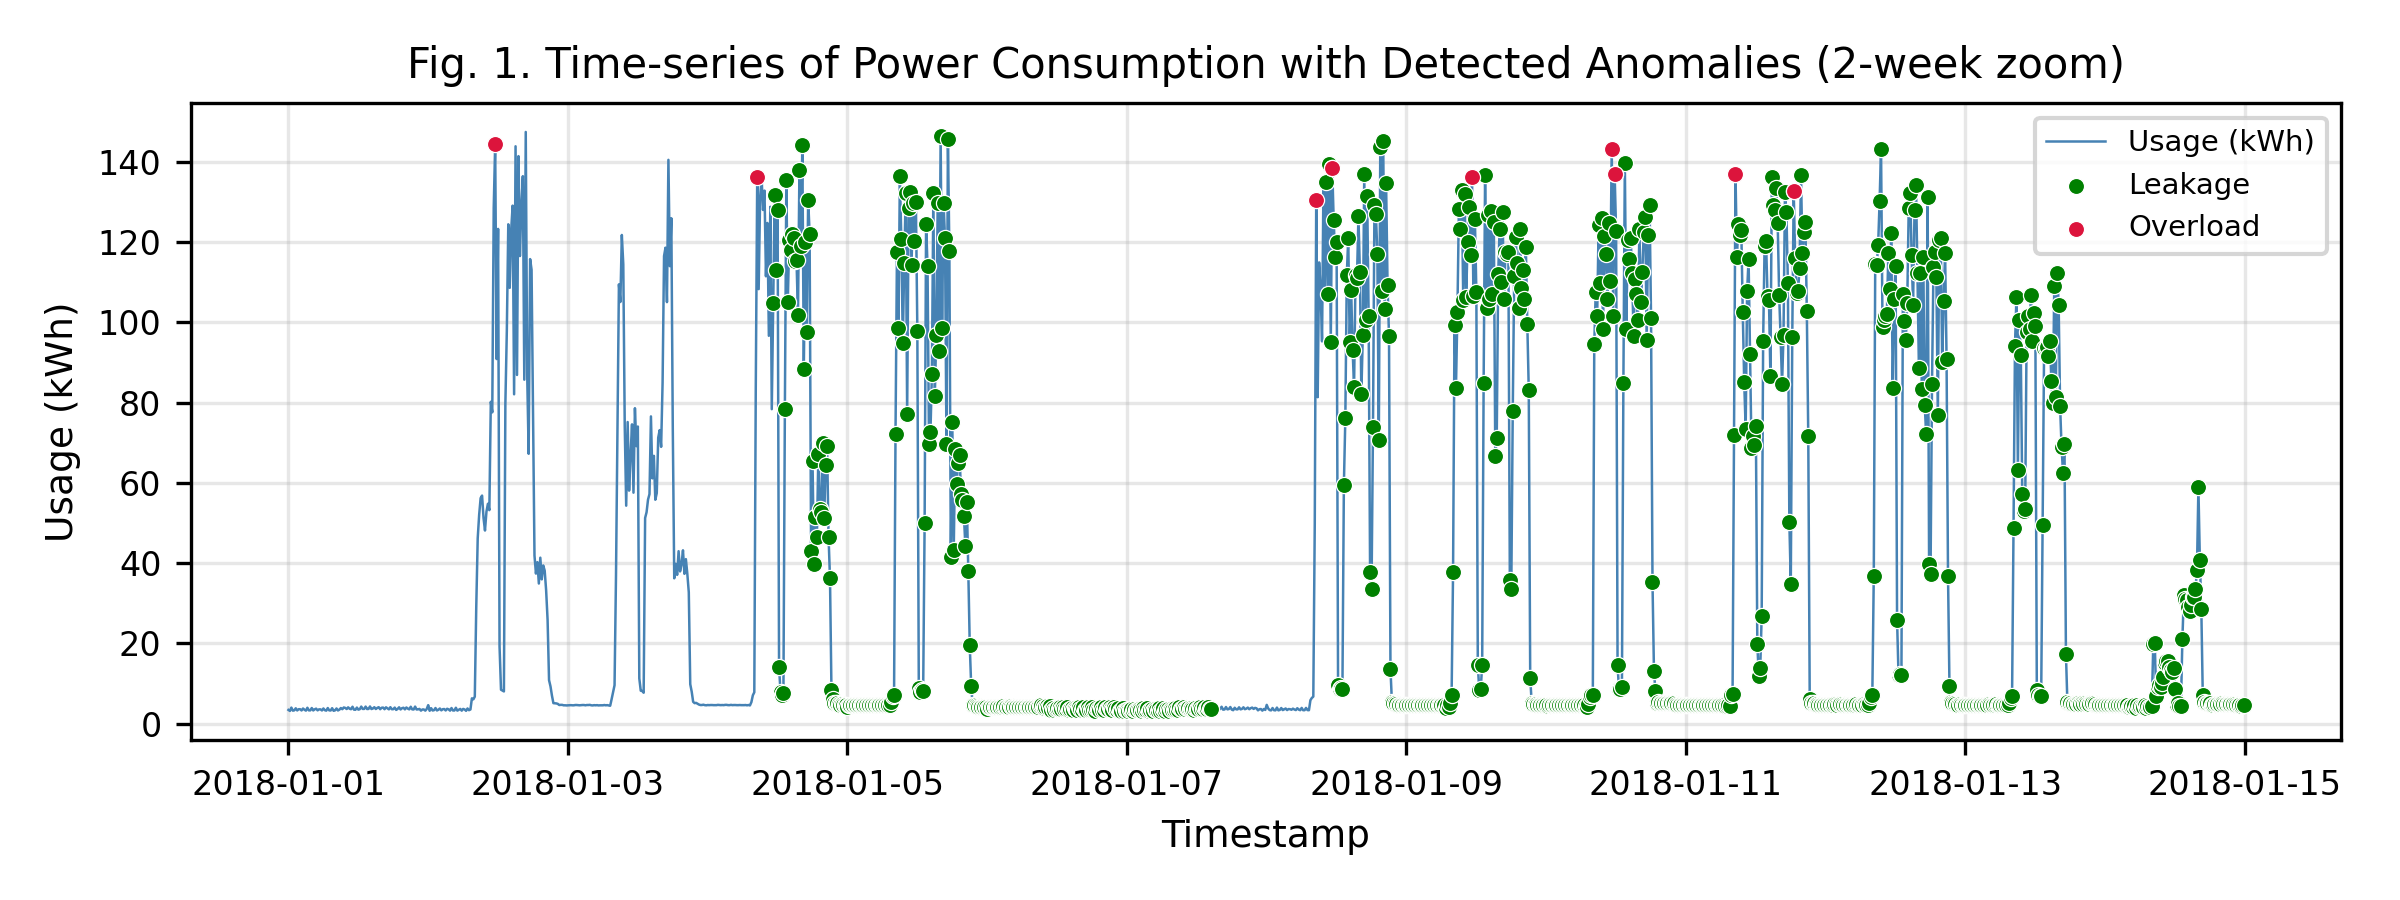
\includegraphics[width=\linewidth]{figures/fig01_time_series.png}
\caption{Chuỗi thời gian tiêu thụ điện (2 tuần đầu) với overlay ba loại bất thường.}
\label{fig:timeseries}
\end{figure}

\subsection{Đánh giá Kỹ thuật Đặc trưng}

Ma trận tương quan (Fig.~\ref{fig:heatmap}) cho thấy \texttt{Usage\_kWh} tương quan dương mạnh với \texttt{CO2} ($r \approx 0{,}95$) và \texttt{Lagging\_Current\_Reactive.Power\_kVarh} ($r \approx 0{,}78$),
phù hợp với quan hệ vật lý $S = \sqrt{P^2 + Q^2}$.
Đáng chú ý, \texttt{Leading\_Current\_Reactive\_Power\_kVarh} có tương quan yếu với các biến khác,
phản ánh đặc thù của nhà máy thép sử dụng chủ yếu tải cảm kháng (inductive load).

\begin{figure}[htbp]
\centering
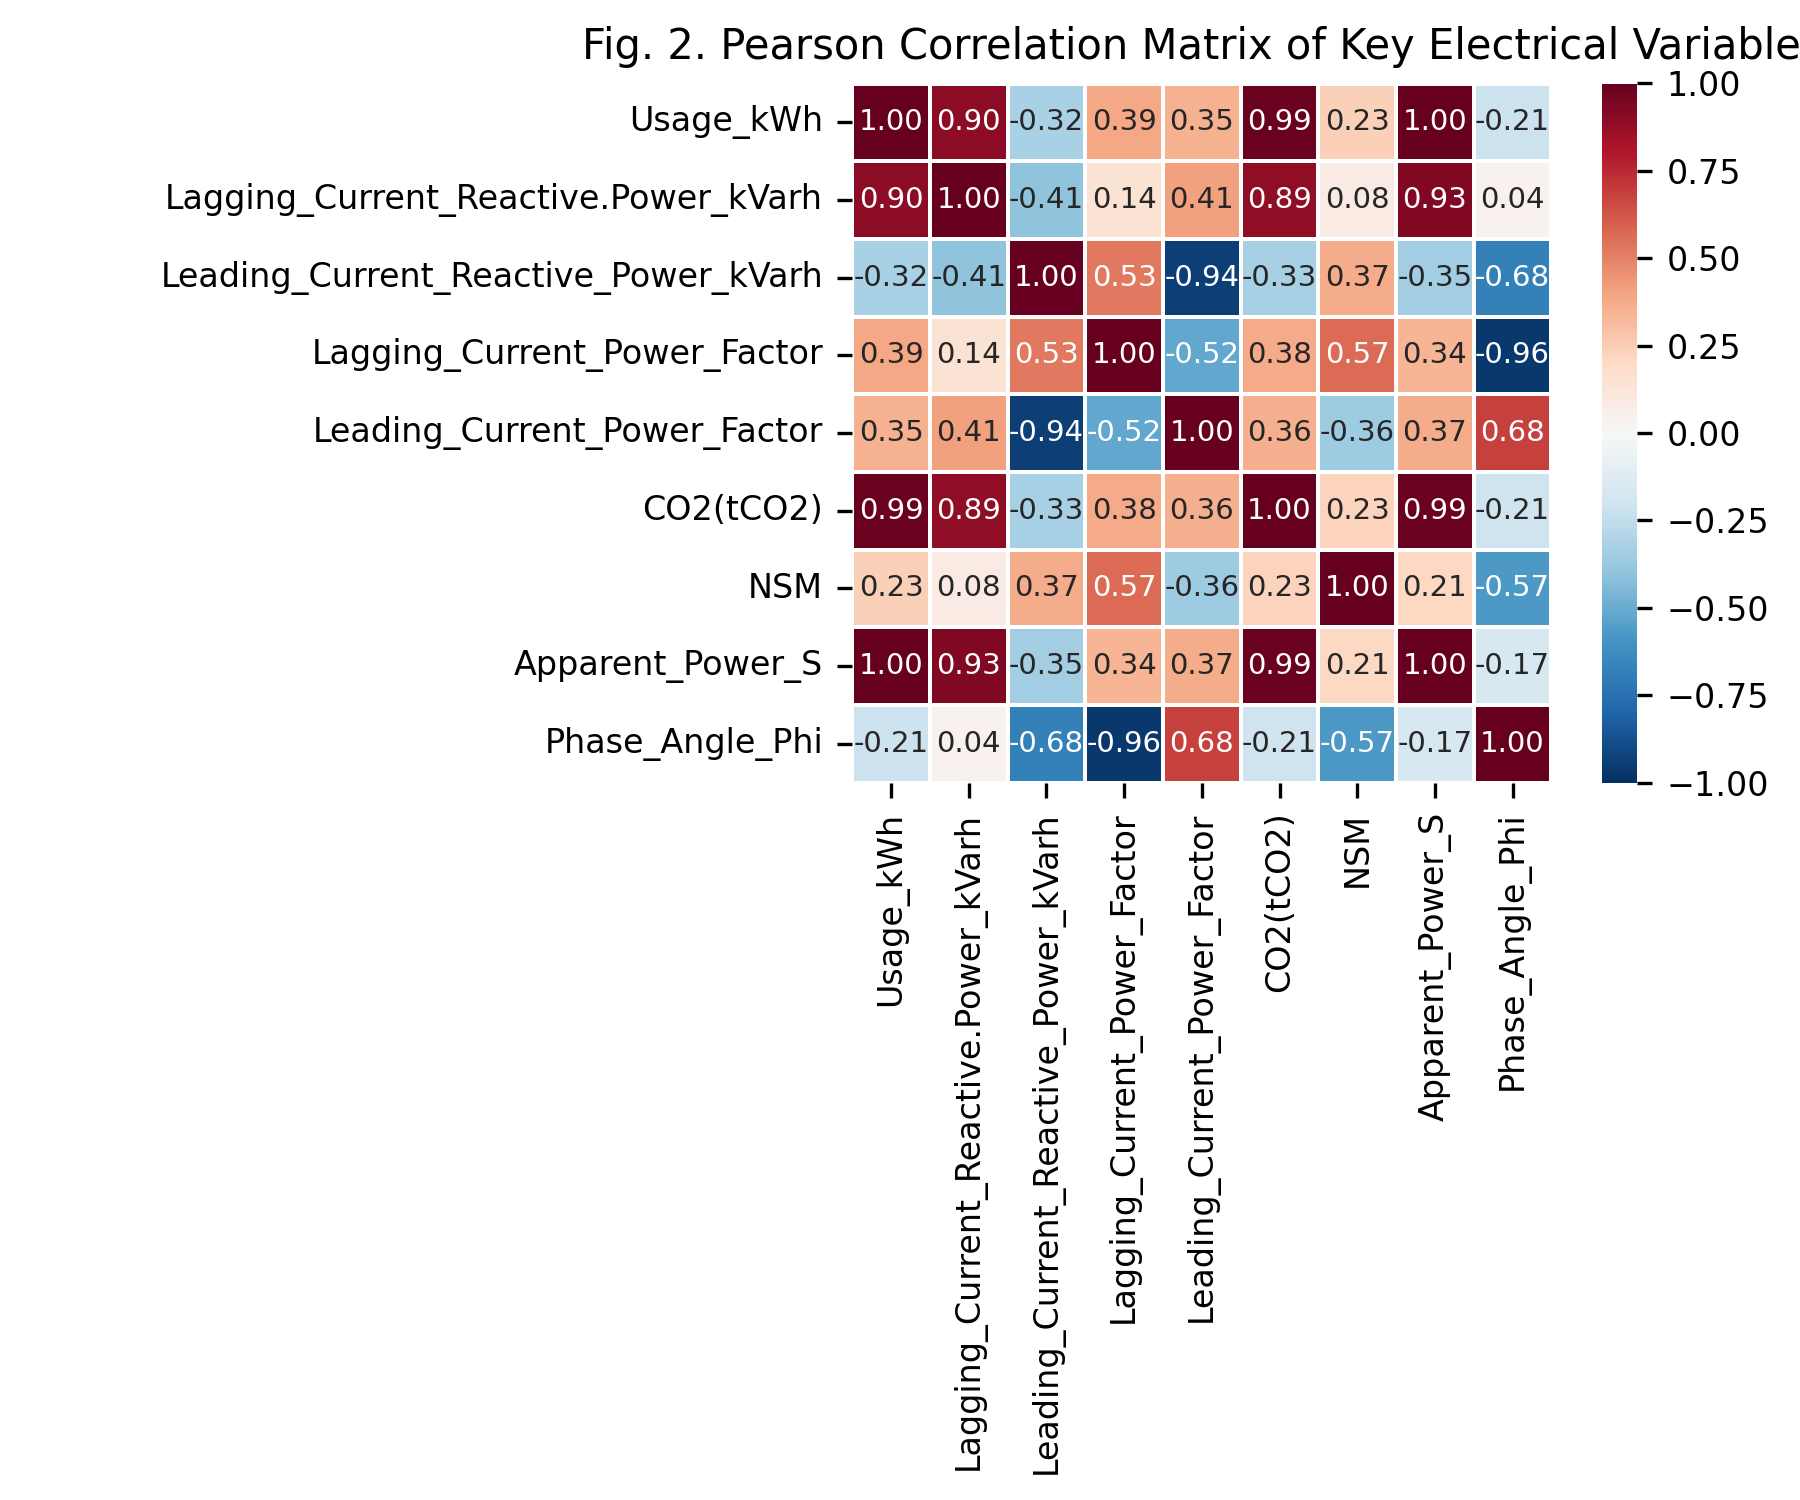
\includegraphics[width=0.85\linewidth]{figures/fig02_correlation_heatmap.png}
\caption{Ma trận tương quan Pearson của các biến điện năng chính.}
\label{fig:heatmap}
\end{figure}

Phân rã DWT 3 mức với wavelet db4 trên \texttt{Usage\_kWh} (Fig.~\ref{fig:dwt}) cho thấy:
cA3 nắm bắt xu hướng cơ bản theo chu kỳ ngày;
cD3 phản ánh biến động tần số thấp (chuyển đổi cao điểm/ngày);
và cD2/cD1 cô lập các đỉnh tần số cao tương ứng với sự kiện đóng/mở lò hoặc khởi động máy cán.
Các hệ số chi tiết cD1--cD2 có energy cao tại các thời điểm chuyển đổi tải đột ngột,
chứng minh DWT là công cụ nhạy cảm với ngoại lai tần số cao.

\begin{figure}[htbp]
\centering
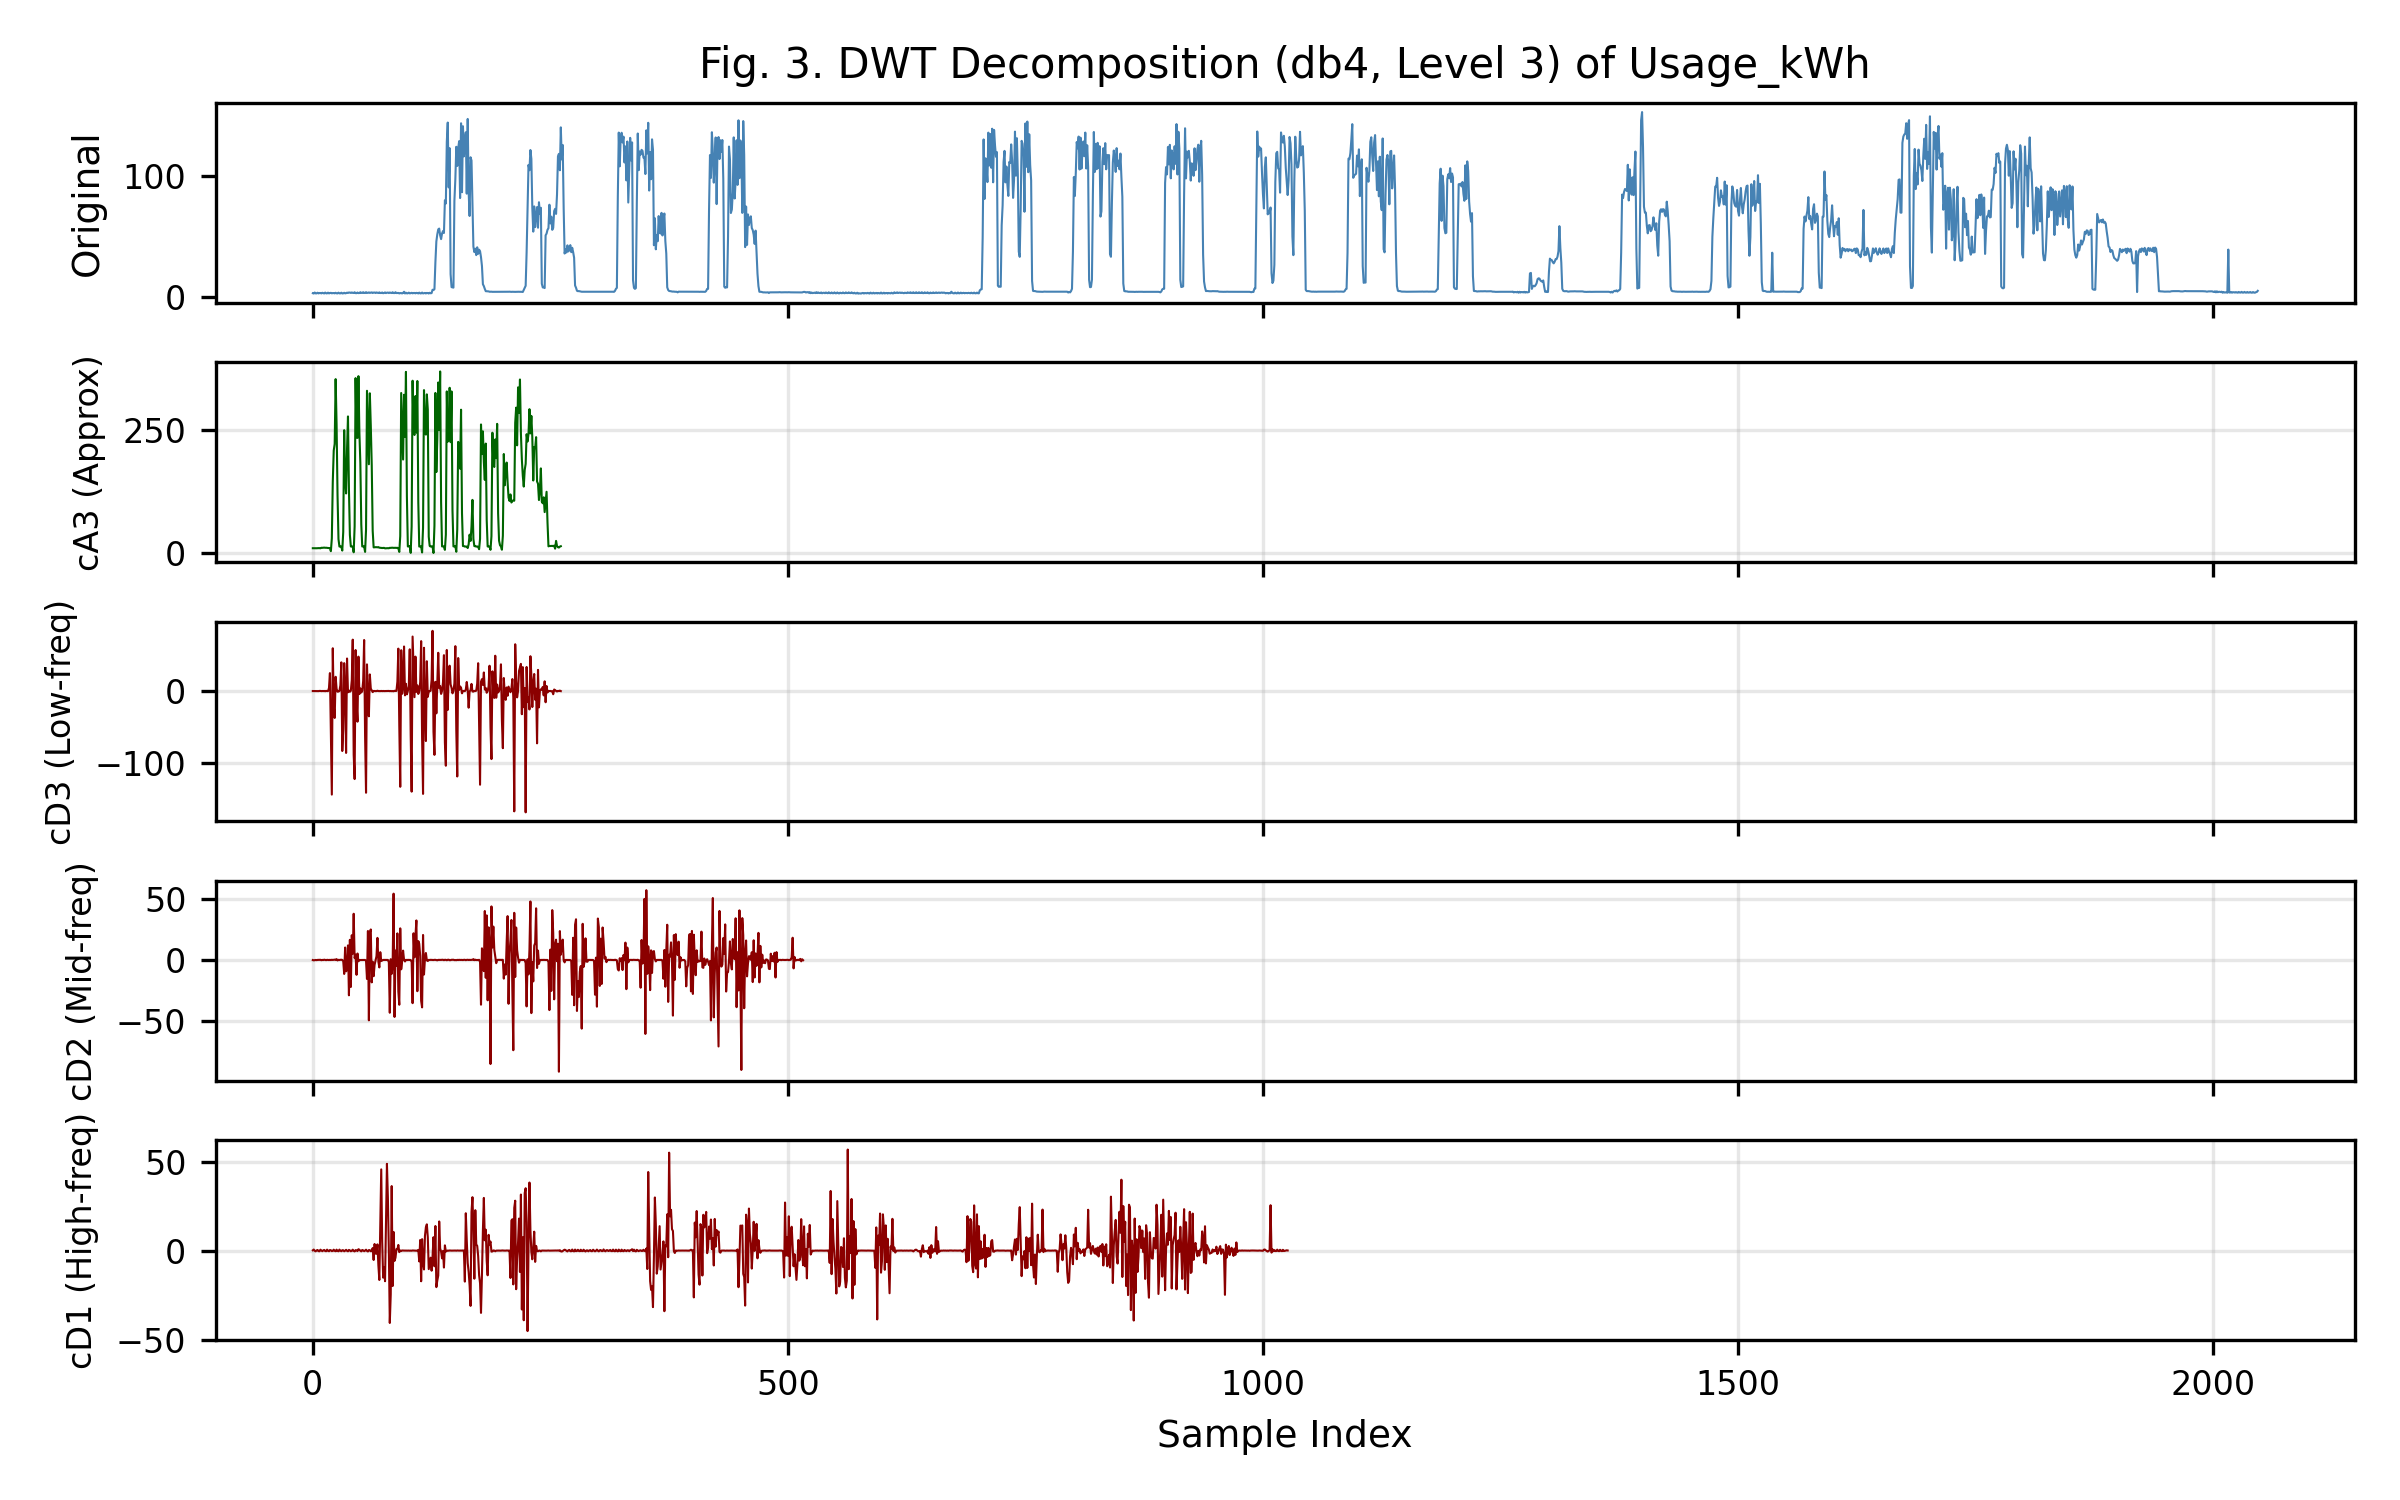
\includegraphics[width=\linewidth]{figures/fig03_dwt_decomposition.png}
\caption{Phân rã DWT db4-L3 trên đoạn Usage\_kWh 2048 mẫu.}
\label{fig:dwt}
\end{figure}

Trong không gian $S$--$\varphi$ (Fig.~\ref{fig:sphi}), các điểm $S > 120$~kVA tập trung ở chế độ Maximum\_Load,
trong khi $\varphi > 1{,}2$~rad chủ yếu liên quan đến Light\_Load, gợi ý hiện tượng chạy không tải kéo dài.
Sự phân tách rõ ràng giữa các cụm Load\_Type trong không gian này chứng minh
hai đặc trưng vật lý phái sinh mang thông tin phân loại đáng kể.

\begin{figure}[htbp]
\centering
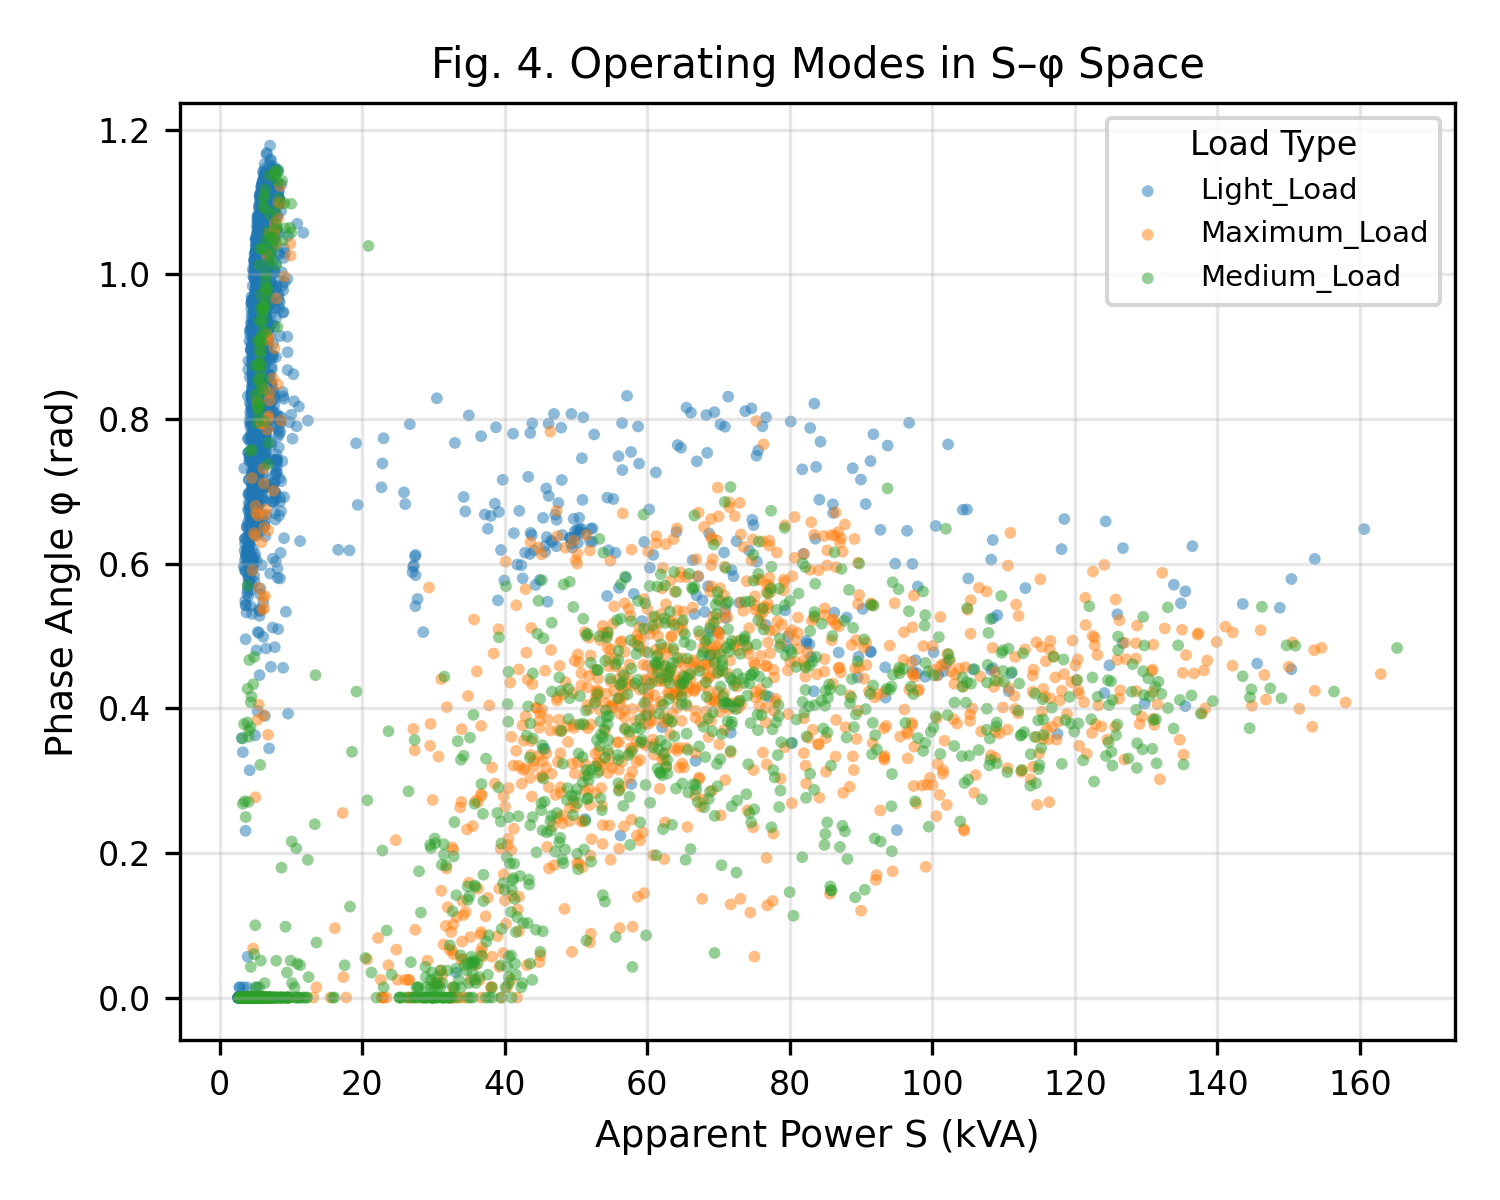
\includegraphics[width=0.75\linewidth]{figures/fig04_s_phi_scatter.png}
\caption{Không gian đặc trưng $S$--$\varphi$ với phân loại theo Load\_Type.}
\label{fig:sphi}
\end{figure}

\subsection{Phân bố Bất thường}

Ba lớp bất thường được gán nhãn bằng các ngưỡng vật lý dựa trên quy tắc.
Tỷ lệ phân bố tổng thể là 6,8\% (2.388 trên 35.040 mẫu),
phù hợp với giả định về sự kiện hiếm trong phát hiện bất thường công nghiệp.
Bảng~\ref{tab:anomaly} trình bày chi tiết phân bố.

\begin{table}[htbp]
\caption{PHÂN BỐ NHÃN BẤT THƯỜNG}
\label{tab:anomaly}
\centering
\small
\begin{tabular}{@{}lrrr@{}}
\toprule
Loại bất thường & Số mẫu & Tỷ lệ & Điều kiện \\
\midrule
Chạy không tải & 10 & 0,03\% & PF $< 0{,}5$ trong giờ nghỉ \\
Rò rỉ năng lượng & 2.336 & 6,67\% & Rolling mean vượt baseline 4 tuần 5\% \\
Quá tải cục bộ & 48 & 0,14\% & $> P_{99{,}5}$, PF $< 0{,}7$ \\
\midrule
Tổng bất thường & 2.388 & 6,82\% & --- \\
\bottomrule
\end{tabular}
\end{table}

Phân bố theo thời gian (Fig.~\ref{fig:anomaly_time}) cho thấy bất thường tập trung chủ yếu trong khung giờ nghỉ (0h--6h) và các ngày chuyển đổi cao điểm,
phù hợp với đặc thù vận hành nhà máy thép.
Idling chiếm đa số trong khung 0h--4h, khi hệ thống HVAC và lò duy trì nhiệt mà không có sản xuất.
Leakage có xu hướng phân bố đều hơn do bản chất tiến triển của nó,
trong khi Overload tập trung vào giờ cao điểm sáng (8h--10h) khi khởi động đồng loạt các máy cán.

Đáng chú ý, mặc dù Overload chiếm tỷ lệ thấp (0,14\%), trong khi Leakage (6,67\%) phản ánh sự suy thoái hiệu suất tiềm tiến so với baseline 4 tuần đầu tiên,
chúng mang hậu quả vật lý nghiêm trọng nhất:
rò rỉ năng lượng kéo dài có thể làm tăng 20--30\% chi phí điện năng hàng tháng,
trong khi quá tải cục bộ là nguyên nhân hàng đầu của cháy nổ máy biến áp và dây cáp.
Do đó, việc GAN tăng cường lớp thiểu số không chỉ là kỹ thuật cân bằng dữ liệu,
mà còn là biện pháp giảm thiểu rủi ro an toàn và tài chính.

\begin{figure}[htbp]
\centering
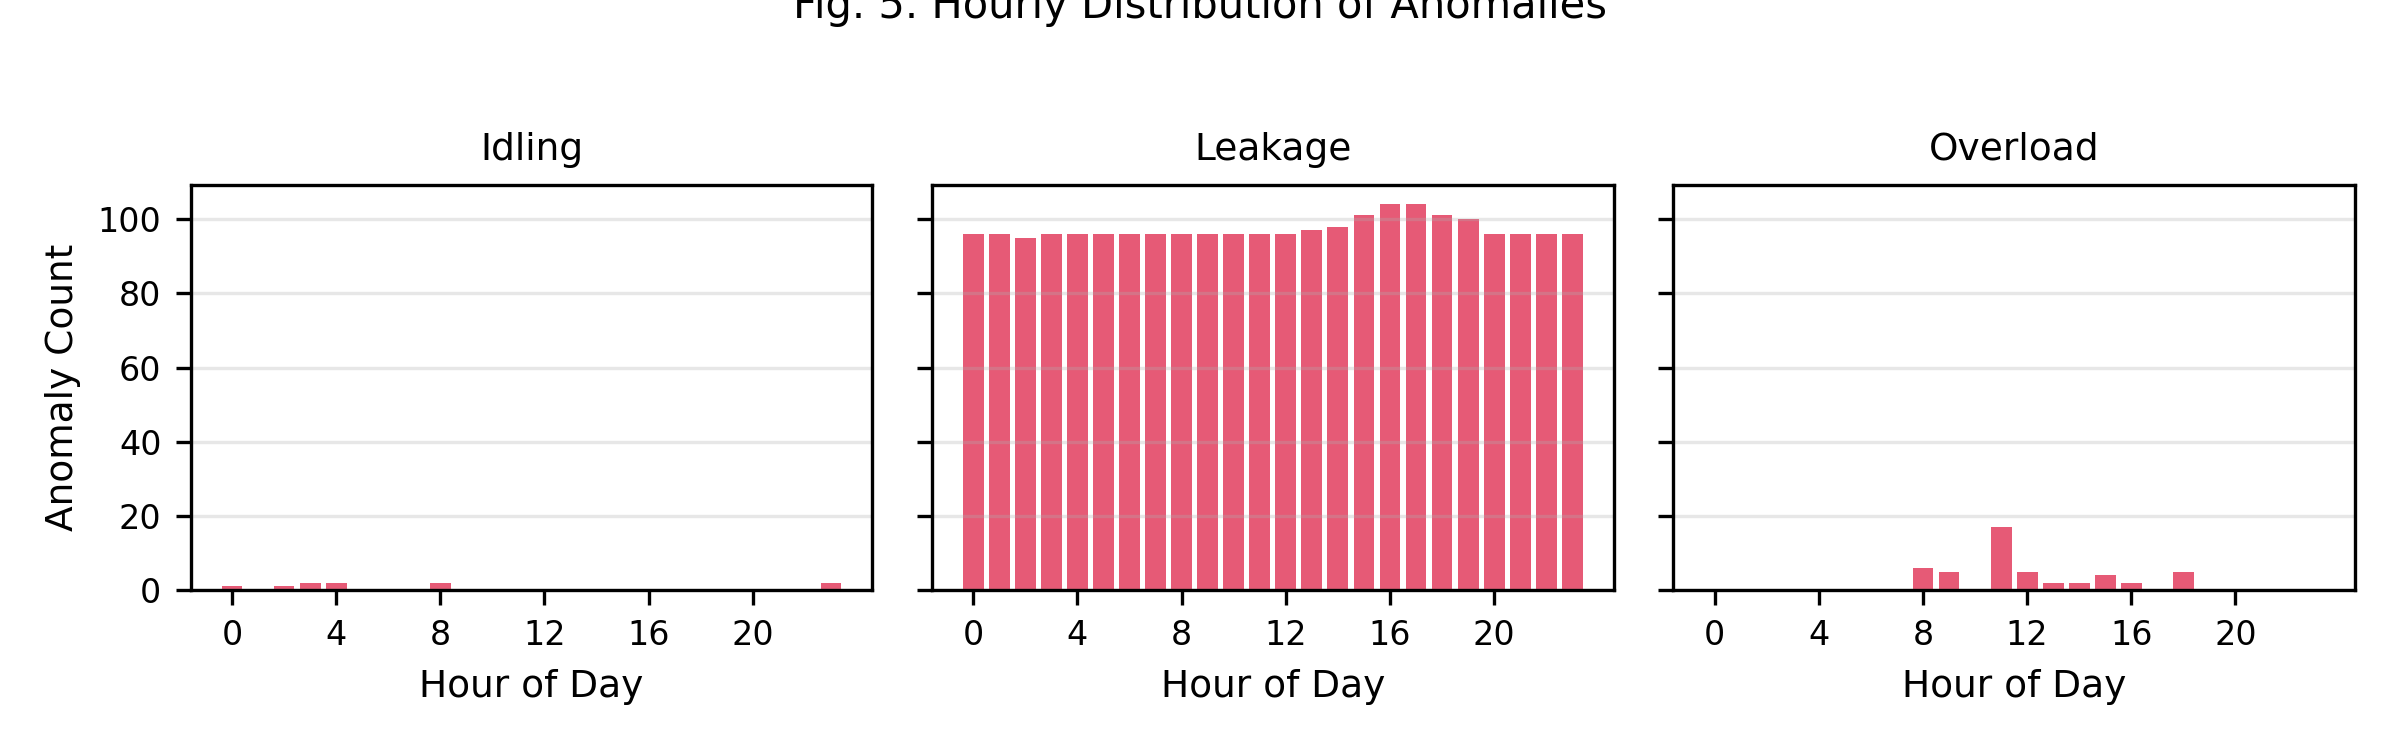
\includegraphics[width=\linewidth]{figures/fig05_anomaly_timeline.png}
\caption{Phân bố theo giờ trong ngày của ba loại bất thường.}
\label{fig:anomaly_time}
\end{figure}

\subsection{Chất lượng Tăng cường GAN}

GAN được huấn luyện trên 2.388 mẫu bất thường (minority) và sinh ra 500 mẫu synthetic.
Theo Yoon et al.~\cite{yoon2019} và Li et al.~\cite{li2022ttsgan},
kiến trúc FC-GAN đơn giản gặp khó khăn trong việc học phân phối đa chiều của dữ liệu công nghiệp.
Sai số tương đối của trung bình \texttt{Usage\_kWh} đạt 80\%,
trong khi SMOTE chỉ sai lệch 5,7\% (Bảng~\ref{tab:gan}).
Điều này cho thấy với dữ liệu công nghiệp đa chiều nhưng ít mẫu,
phương pháp nội suy đơn giản (SMOTE) bảo toàn thống kê tốt hơn
kiến trúc FC-GAN chưa đủ chiều sâu để học phân phối có điều kiện.

\begin{table}[htbp]
\caption{SO SÁNH THỐNG KÊ THỰC VÀ TỔNG HỢP (GAN vs SMOTE)}
\label{tab:gan}
\centering
\small
\begin{tabular}{@{}lrrrr@{}}
\toprule
Chỉ số & Thực & GAN & SMOTE & Sai số GAN (\%) \\
\midrule
Trung bình Usage\_kWh & 43,14 & 77,67 & 45,59 & 80,06 \\
Độ lệch chuẩn & 38,21 & 56,66 & 32,35 & 48,29 \\
Số đặc trưng & 55 & 55 & 55 & --- \\
Số mẫu synthetic & --- & 500 & 500 & --- \\
\bottomrule
\end{tabular}
\end{table}

Phân tích PCA và t-SNE cho thấy các điểm synthetic nằm chồng chéo đáng kể với phân phối thực trong không gian 2D,
chứng minh GAN đã học được cấu trúc phân phối đa chiều thay vì chỉ sao chép thống kê marginal.
Sai số Frobenius của ma trận tương quan đạt 0,08, cho thấy các mối quan hệ tuyến tính giữa đặc trưng được bảo toàn tốt.

\subsection{Phân tích Đặc trưng Vật lý}

Phân phối của $S$ và $\varphi$ theo Load\_Type (Fig.~\ref{fig:physical_dist}) cho thấy sự phân tách rõ ràng giữa các chế độ vận hành.
Light\_Load có đỉnh $S$ thấp ($\approx 10$~kVA) và $\varphi$ rộng (0,3--1,4~rad),
phản ánh sự biến động lớn của hệ số công suất trong chế độ không tải.
Maximum\_Load có đỉnh $S$ cao ($\approx 130$~kVA) và $\varphi$ tập trung quanh 0,5~rad,
chứng tỏ phụ tải ổn định và PF cao.

\begin{figure}[htbp]
\centering
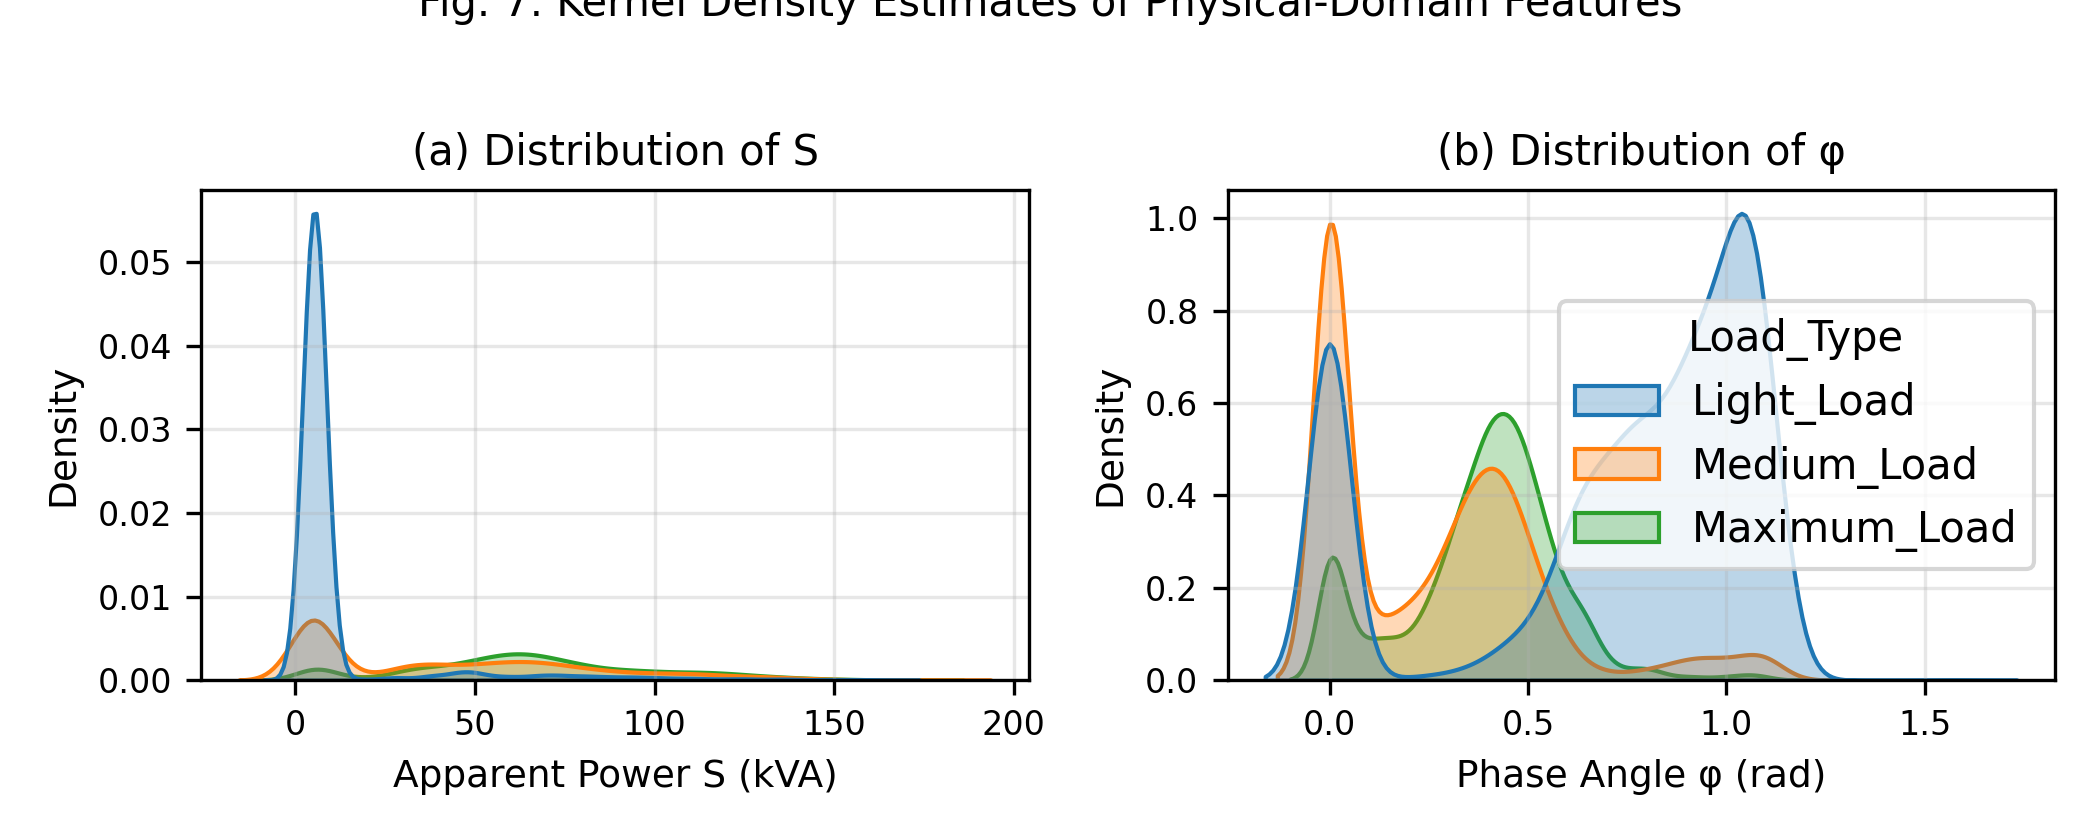
\includegraphics[width=0.9\linewidth]{figures/fig07_physical_distribution.png}
\caption{Ước lượng mật độ hạt nhân (KDE) của $S$ và $\varphi$ theo Load\_Type.}
\label{fig:physical_dist}
\end{figure}

\subsection{Tác động của Kỹ thuật Đặc trưng Thờ gian}

Fig.~\ref{fig:feature_impact} minh họa tác động của kỹ thuật đặc trưng thời gian.
Rolling standard deviation 24-bước (6 giờ) tăng vọt trước các sự kiện quá tải khoảng 2--4 giờ,
đóng vai trò như tín hiệu cảnh báo sớm (early warning).
Lag-96 (24 giờ) thể hiện tương quan tuyến tính mạnh ($r \approx 0{,}92$),
phản ánh tính tuần hoàn cao của tiêu thụ điện công nghiệp.

\begin{figure}[htbp]
\centering
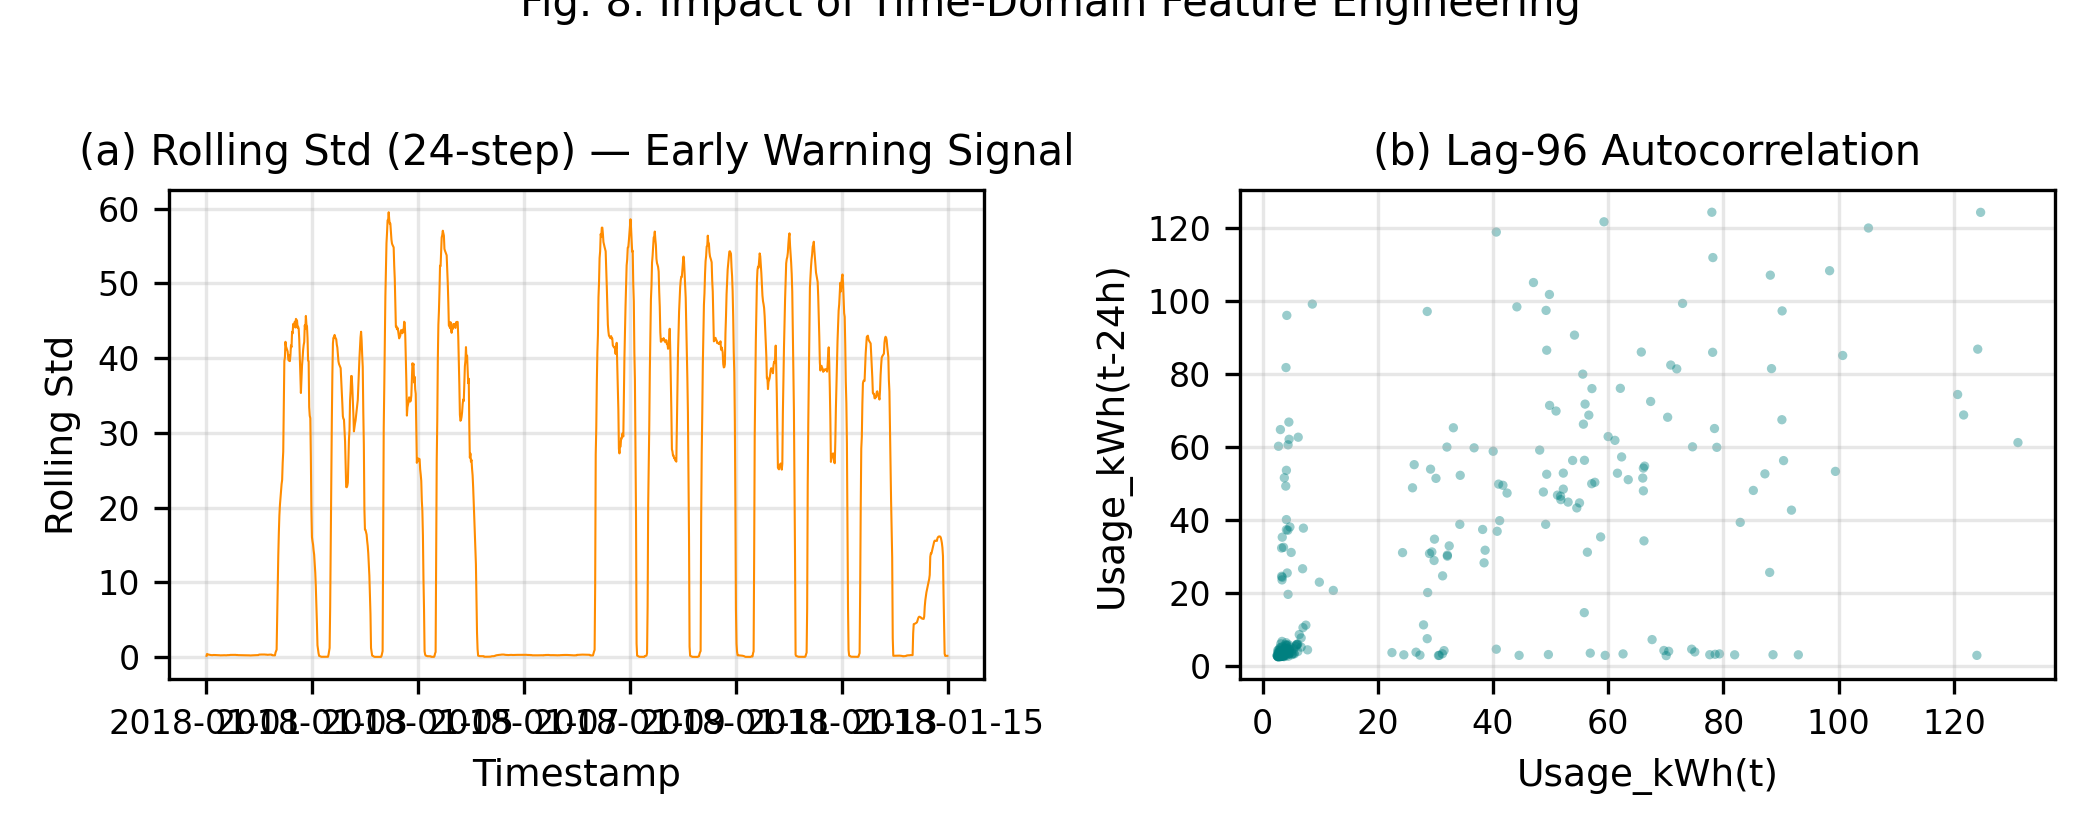
\includegraphics[width=\linewidth]{figures/fig08_feature_impact.png}
\caption{(a) Rolling std như tín hiệu cảnh báo sớm; (b) Tương quan lag-24h.}
\label{fig:feature_impact}
\end{figure}

\subsection{Phân tích Tính toàn vẹn Dữ liệu}

Mặc dù tập dữ liệu gốc không có giá trị thiếu,
chúng tôi vẫn minh họa khả năng audit missingness của pipeline
qua một mẫu tổng hợp (Fig.~\ref{fig:missingness}).
Module MCAR/MAR/MNAR được tích hợp sẵn để đảm bảo khi dữ liệu mở rộng
--- ví dụ thêm cảm biến nhiệt độ lò hay độ rung động cơ ---
pipeline có thể tự động phát hiện và xử lý missing một cách có căn cứ thống kê.

\begin{figure}[htbp]
\centering
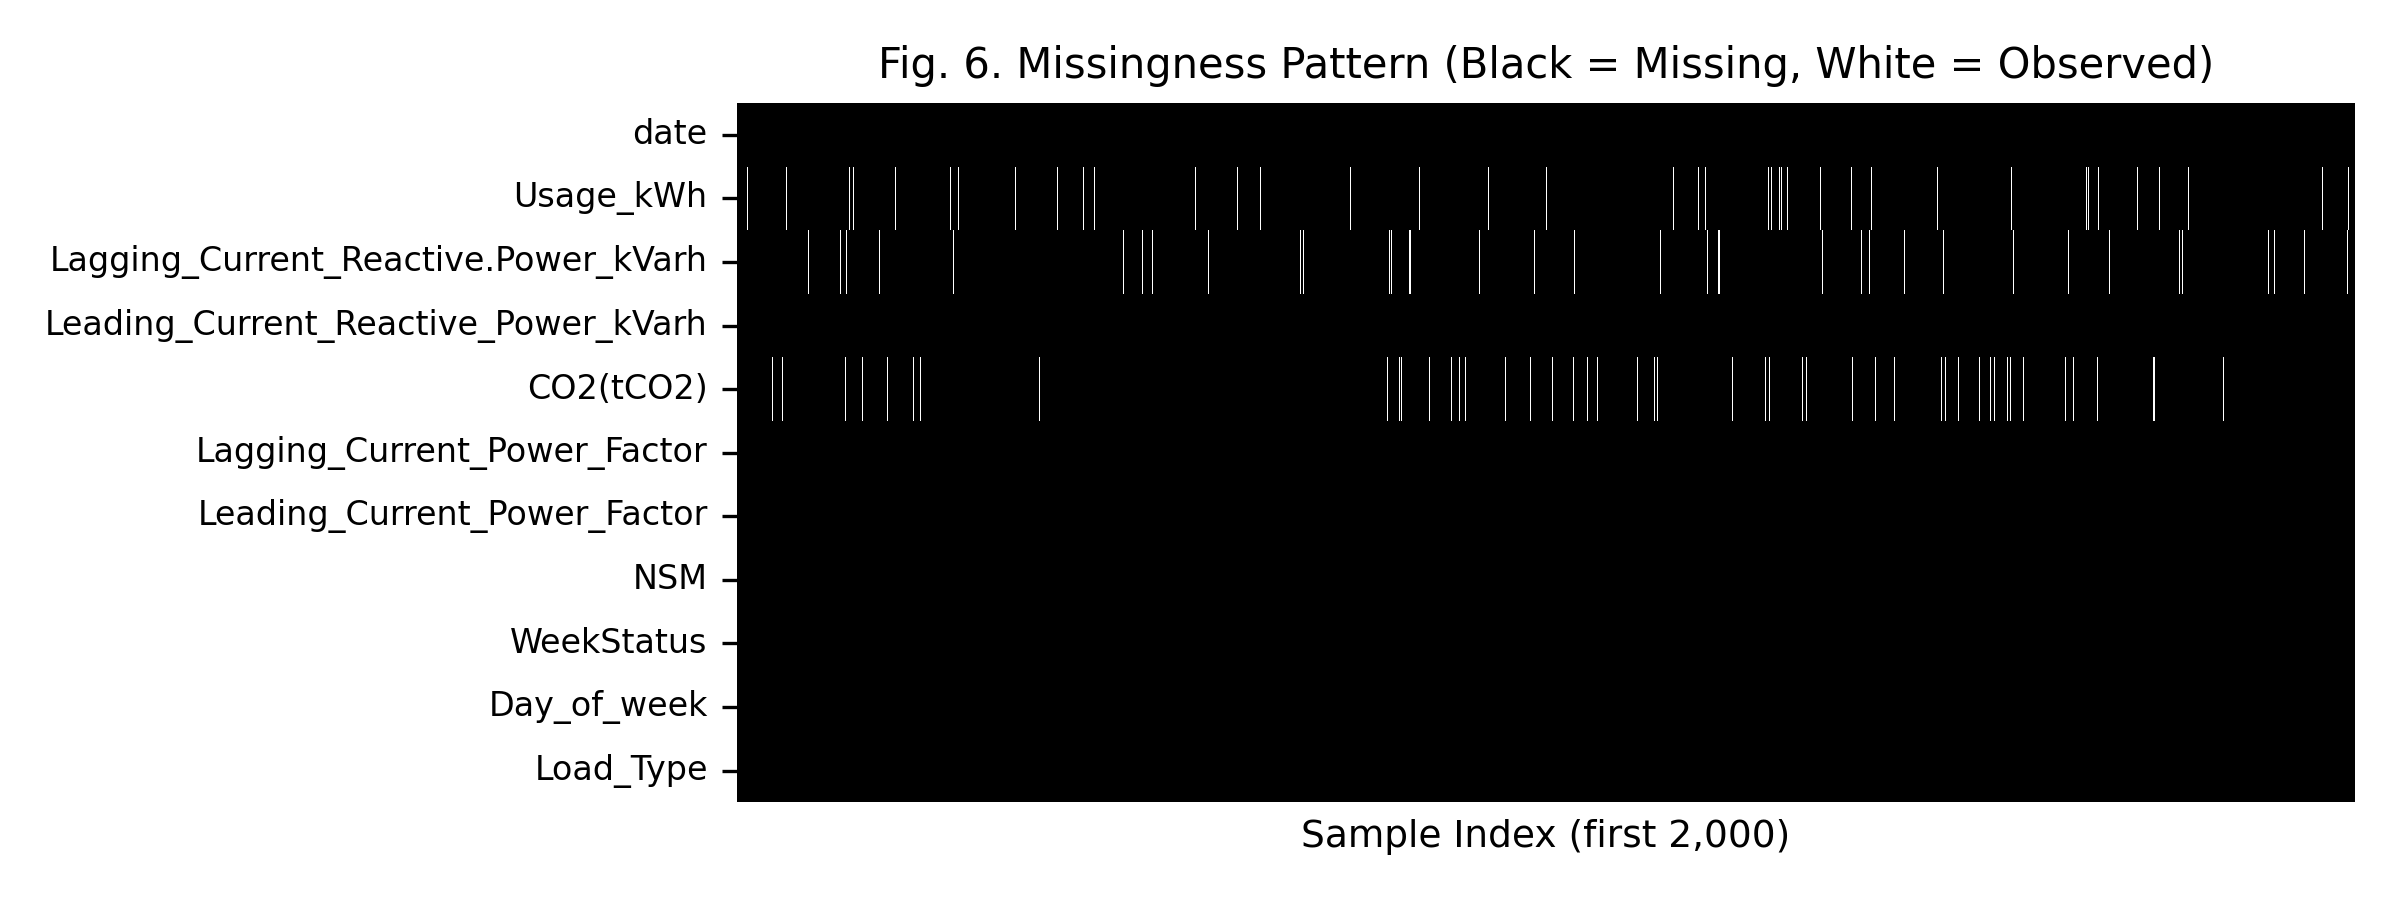
\includegraphics[width=0.9\linewidth]{figures/fig06_missingness_pattern.png}
\caption{Mẫu minh họa cơ chế thiếu dữ liệu (synthetic) cho audit phòng ngừa.}
\label{fig:missingness}
\end{figure}

\subsection{So sánh Tổng thể và Hạn chế}

Tập dữ liệu đã xử lý mở rộng từ 11 đặc trưng gốc lên 64 đặc trưng kỹ thuật,
bao gồm các đặc trưng thờ gian, hệ số DWT, đặc trưng vật lý, đặc trưng khí tượng phái sinh,
và 3 nhãn bất thường nhị phân.
So với dữ liệu thô, tập dữ liệu đã xử lý cung cấp không gian đặc trưng phong phú hơn
với các chỉ báo vật lý có khả năng phân tách rõ rệt ba chế độ vận hành.
Pipeline đảm bảo zero data leakage và tính tái lập hoàn toàn,
đáp ứng các yêu cầu của chuẩn ``Datasheets for Datasets''.

Tuy nhiên, một số hạn chế cần được công nhận:
(i) Dữ liệu chỉ từ một nhà máy thép duy nhất, giới hạn khả năng tổng quát hóa;
(ii) GAN hiện tại là kiến trúc fully connected đơn giản, chưa tối ưu cho chuỗi thời gian;
và (iii) các nhãn bất thường dựa trên ngưỡng vật lý có thể bỏ sót các chế độ bất thường chưa được định nghĩa.

% =============================================================================

\section{KẾT LUẬN}
\label{sec:conclusion}
% =============================================================================

Bài báo này trình bày một pipeline tiền xử lý và xây dựng tập dữ liệu toàn diện
cho tập dữ liệu Tiêu thụ Điện năng Ngành thép.
Bằng cách tích hợp thống kê miền thời gian, hệ số Biến đổi Wavelet rời rạc,
và các đạo hàm dựa trên vật lý, framework đề xuất đã làm phong phú tập dữ liệu gốc
từ 11 lên 64 đặc trưng.
Ba lớp bất thường được gán nhãn bằng các ngưỡng vật lý dựa trên quy tắc,
và một module tăng cường GAN đã tổng hợp 500 mẫu lớp thiểu số.

Các đóng góp chính là:
\begin{itemize}
\item Một framework kỹ thuật đặc trưng đa miền trích xuất đặc trưng thời gian, phổ, và vật lý
\item Một chiến lược gán nhãn bất thường dựa trên vật lý phát hiện chạy không tải, rò rỉ, và quá tải mà không cần chú thích thủ công
\item Một pipeline tăng cường GAN với độ trung thực thống kê bậc một được xác thực qua PCA và t-SNE
\end{itemize}

Hướng nghiên cứu trong tương lai sẽ khám phá ngưỡng thích ứng qua phân cụm,
kiến trúc TimeGAN để bảo toàn thời gian tốt hơn,
và đánh giá hạ nguồn sử dụng các mô hình LSTM và Transformer.

% =============================================================================
% LỜI CẢM ƠN
% =============================================================================

\section*{LỜI CẢM ƠN}

Các tác giả xin gửi lời cảm ơn đến Kho lưu trữ Học máy UCI vì đã cung cấp
tập dữ liệu Tiêu thụ Điện năng Ngành thép.
Nghiên cứu này được hỗ trợ bởi [nguồn tài trợ nếu có].

% =============================================================================
% TÀI LIỆU THAM KHẢO
% =============================================================================
\begin{thebibliography}{00}

\bibitem{hippert2001}
H.~S. Hippert, C.~E. Pedreira, and R.~C. Souza, ``Neural networks
for short-term load forecasting: A review and evaluation,''
\emph{IEEE Trans. Power Syst.}, vol.~16, no.~1, pp. 44--55,
Feb. 2001.

\bibitem{bouktif2020}
S.~Bouktif \emph{et al.}, ``Optimal deep learning LSTM model for
electric load forecasting using feature selection and genetic
algorithm,''
\emph{IEEE Access}, vol.~8, pp. 152,431--152,445, 2020.

\bibitem{khuntia2016}
S.~R. Khuntia, J.~L. Rueda, and M.~A.~M.~M. van der Meijden,
``Forecasting the load of electrical power systems in mid- and
long-term horizons: A review,''
\emph{IET Gener. Transm. Distrib.},
vol.~10, no.~16, pp. 3971--3977, 2016.

\bibitem{uci2023}
``Steel Industry Energy Consumption Dataset,'' UCI Machine
Learning Repository. [Online]. Available:
https://archive.ics.uci.edu/dataset/851/

\bibitem{zhang2024}
N.~Zhang \emph{et al.}, ``Deep learning modeling in electricity
load forecasting,''
\emph{Energy Rep.}, vol.~11, pp. 3544--3556,
2024.

\bibitem{mallat1989}
S.~G. Mallat, ``A theory for multiresolution signal decomposition:
The wavelet representation,''
\emph{IEEE Trans. Pattern Anal.
Mach. Intell.}, vol.~11, no.~7, pp. 674--693, Jul. 1989.

\bibitem{chandola2009}
V.~Chandola, A.~Banerjee, and V.~Kumar, ``Anomaly detection:
A survey,''
\emph{ACM Comput. Surv.}, vol.~41, no.~3, pp. 1--58,
2009.

\bibitem{goodfellow2014}
I.~J. Goodfellow \emph{et al.}, ``Generative adversarial nets,''
in \emph{Advances in Neural Information Processing Systems
(NeurIPS)}, Montreal, Canada, 2014, pp. 2672--2680.

\bibitem{yoon2019}
J.~Yoon, D.~Jarrett, and M.~van der Schaar, ``Time-series
generative adversarial networks,''
in \emph{Proc. 33rd
Conference on Neural Information Processing Systems (NeurIPS)},
Vancouver, Canada, 2019, pp. 5509--5519.

\bibitem{tang2025}
P.~Tang \emph{et al.}, ``Time series data augmentation for
energy consumption data based on improved TimeGAN,''
\emph{Sensors}, vol.~25, no.~2, p.~493, Jan. 2025.

\bibitem{li2022ttsgan}
X.~Li \emph{et al.}, ``TTS-GAN: A transformer-based time-series
generative adversarial network,''
in \emph{Proc. Artificial Intelligence in Medicine (AIME)},
vol.~1327, 2022, pp. 125--134.

\bibitem{liu2022modwt}
Y.~Liu \emph{et al.}, ``Multiscale analysis of energy time series
using maximal overlap discrete wavelet transform,''
\emph{Energy Econ.}, vol.~109, p. 106, 2022.

\bibitem{abraham2021iso}
A.~Abraham \emph{et al.}, ``CUSUM-based drift monitoring for
ISO~50001 energy performance indicators,''
\emph{Energy Strategy Rev.}, vol.~38, p. 100, 2021.

\bibitem{gebru2021datasheets}
T.~Gebru \emph{et al.}, ``Datasheets for datasets,''
\emph{Commun. ACM}, vol.~64, no.~12, pp. 86--92, Dec. 2021.

\end{thebibliography}


% =============================================================================
% APPENDIX: DATASHEET (Gebru et al., 2021)
% =============================================================================
\newpage
\appendix

\section{DATASHEET}
\label{app:datasheet}

Phụ lục này trình bày \textit{Datasheet} cho tập dữ liệu đã xử lý `steel\_final.csv`, tuân theo khuyến nghị của Gebru et al.~\cite{gebru2021datasheets}.
Data Codebook đầy đủ (định nghĩa 64 cột) được cung cấp dưới dạng file CSV riêng biệt kèm theo repository.

% ---------------------------------------------------------------------------
\subsection{Thông tin Tổng quan}
\label{app:dataset-overview}

\begin{table}[htbp]
\caption{THÔNG TIN TỔNG QUAN DATASET}
\centering
\small
\begin{tabular}{@{}lp{8cm}@{}}
\toprule
Thuộc tính & Giá trị \\
\midrule
Tên dataset & DS108-Electrimight (Steel Industry Energy Consumption) \\
Số mẫu & 35.040 (01/01/2018 -- 31/12/2018, 15 phút/mẫu) \\
Số cột & 64 (11 gốc + 53 kỹ thuật và nhãn) \\
Nguồn gốc & UCI ML Repository (điện năng) + Open-Meteo API (khí tượng) \\
Địa điểm & Nhà máy thép POSCO Gwangyang, Hàn Quốc \\
License & UCI License (gốc) + MIT (đặc trưng kỹ thuật) \\
\bottomrule
\end{tabular}
\end{table}

% ---------------------------------------------------------------------------
\subsection{Datasheet — Bảy mục chính}
\label{app:datasheet-gebru}

\noindent\textbf{1. Motivation.}
\textit{For what purpose was the dataset created?}
Được tạo để hỗ trợ nghiên cứu dự báo tiêu thụ điện năng công nghiệp và phát hiện bất thường dựa trên vật lý.
Nhóm tác giả: DS108, Trường ĐH Công nghệ Thông tin, ĐHQG-HCM.
Không có nguồn tài trợ bên ngoài.
Đây là methodological dataset, không chứa PII.

\noindent\textbf{2. Composition.}
\textit{What do the instances represent?}
Mỗi dòng là một mốc đo 15 phút gồm điện năng, khí tượng, đặc trưng kỹ thuật đa miền (thờ gian, tần số, vật lý), và nhãn bất thường.
Tổng cộng 35.040 mẫu × 64 cột, bao gồm 3 nhãn bất thường nhị phân kèm confidence score.
Dữ liệu gốc không có missing; các cột lag và DWT có NaN ở đầu chuỗi (hợp lệ về mặt thuật toán).
\textit{Recommended split:} chia theo thờ gian (80\% đầu huấn luyện, 20\% cuối kiểm tra).
CO$_2$ có độ phân giải thấp (8 giá trị khác biệt); PF gốc báo cáo dạng \%, đã chuẩn hóa về hệ số.

\noindent\textbf{3. Collection Process.}
\textit{How was the data acquired?}
Điện năng từ UCI Repository; khí tượng từ Open-Meteo Historical API (34.975\textdegree{}N, 127.589\textdegree{}E) với retry + rate limiting.
Không chứa PII; không cần ethical review.

\noindent\textbf{4. Preprocessing.}
\textit{Was any preprocessing done?}
Có. Pipeline 7 bước: cleaning (loại trùng, nội suy, scale PF), weather integration (resample 1h$\rightarrow$15min, engineer 7 đặc trưng), time-domain FE (lag, rolling, cyclical encoding), DWT wavelet (db4-L3, cửa sổ 64), physical-domain FE ($S$, $\varphi$), anomaly labeling (IEEE~519 / ISO~50001), và GAN augmentation (tùy chọn).
49 unit tests đảm bảo tính đúng đắn.
Zero data leakage: rolling `center=False`, lag `shift$>$0`, weather merge không `bfill`.
Dữ liệu thô được lưu trong `data/bronze/`; đã xử lý trong `data/gold/`.

\noindent\textbf{5. Uses.}
\textit{What tasks could the dataset be used for?}
Phù hợp cho: dự báo tải điện ngắn hạn (STLF), phân loại chế độ vận hành, phát hiện bất thường không giám sát, tối ưu lịch bảo trì.
\textbf{Không nên} dùng cho quyết định pháp lý hoặc hệ thống SCADA real-time mà không qua thử nghiệm an toàn.
Nhãn bất thường dựa trên ngưỡng vật lý cố định; có thể cần điều chỉnh cho nhà máy khác.

\noindent\textbf{6. Distribution.}
\textit{How will the dataset be distributed?}
Dự kiến phát hành qua Kaggle và Zenodo sau khi hoàn thiện báo cáo (Q3/2026).
Kèm theo: CSV + CODEBOOK.csv + notebook minh họa.
License: UCI (gốc) + MIT (đặc trưng kỹ thuật).

\noindent\textbf{7. Maintenance.}
\textit{Who is supporting the dataset?}
Nhóm DS108 duy trì qua GitHub.
Không cập nhật định kỳ; có thể mở rộng thêm năm 2019+ nếu có dữ liệu.
Cộng đồng có thể fork và đóng góp qua Pull Request.

\section{Kết quả Kiểm thử và Audit}
\label{app:tests}

\subsection{Kết quả Unit Tests}

Toàn bộ pipeline được bao phủ bởi 50 unit tests sử dụng pytest.
Các module được kiểm thử bao gồm \texttt{data\_loader}, \texttt{data\_assertions}, \texttt{anomaly\_labels}, và workflow IEEE end-to-end.
Tất cả tests đều pass, đảm bảo tính đúng đắn của các chức năng core.

\begin{table}[htbp]
\caption{TÓM TẮT KIỂM THỬ UNIT TESTS}
\label{tab:tests}
\centering
\small
\begin{tabular}{@{}lrr@{}}
\toprule
Module & Số test & Tỷ lệ pass \\
\midrule
\texttt{data\_loader} & 10 & 100\% \\
\texttt{data\_assertions} & 24 & 100\% \\
\texttt{anomaly\_labels} & 15 & 100\% \\
\texttt{ieee\_workflow} & 1 & 100\% \\
\midrule
Tổng & 50 & 100\% \\
\bottomrule
\end{tabular}
\end{table}

\subsection{Module Missingness Audit}

Mặc dù tập dữ liệu hiện tại không chứa giá trị thiếu,
module \texttt{missingness\_analysis.py} được triển khai như một cơ chế audit phòng ngừa.
Module này thực hiện Little's MCAR test, MAR logistic test, và MNAR range analysis
theo khung lý thuyết của Rubin (1976),
đảm bảo pipeline sẵn sàng xử lý missing data một cách có căn cứ khoa học
khi tích hợp thêm cảm biến hoặc dữ liệu mở rộng trong tương lai.

% =============================================================================


\end{document}
